\chapter{Design og implementering}

\section{Software Design}

\subsection{SPI Devkit 8000 - Candygun driver}

Candygun driveren sørger for SPI-kommunikationen fra Devkit8000 til PSoC0. Derved kan der sendes kommandoer og aflæses information fra PSoC0. Devkit 8000 fungerer som master og vil altid være den, der initierer en tranfer. 

\subsubsection{Indstillinger for SPI}
Indstilnger for SPI-kommunikationen ses i tabel \ref{SPItabel}. SPI-kommunikationen er implementeret med SPI bus nummer 1, SPI chip-select 0 og en hastighed på 1 MHz (et godt stykke under max på 20 MHz for en sikkerhedsskyld). Desuden starter clocken højt og data ændres på falling edge og aflæses på rising edge. Dermed bliver SPI Clock Mode 3. Derudover sendes der 8 bit pr transmission, hvilket passer med SPI-protokollen for projektet.\\

\begin{table}[H]
	\centering
	\caption{Indstillinger for SPI}
	\label{SPItabel}
	\begin{tabular}{|l|l|}
		\hline
		\textbf{Indstillingsparameter} & \textbf{Værdi} \\ \hline
		SPI bus nr.                    & 1              \\ \hline
		SPI chip-select                & 0              \\ \hline
		Hastighed                      & 1 MHz          \\ \hline
		SPI Clock Mode                 & 3              \\ \hline
		Bit per transmission           & 8              \\ \hline
	\end{tabular}
\end{table}


\subsubsection{Opbygning af driver}
Selve driveren er i candygun.c opbygget som en char driver. For at holde forskellige funktionaliteter adskilt er alle funktioner, der har med SPI at gøre, implementeret i filen candygun-spi-c. Så når der fx skal requestes en SPI ressource i init-funktionen i candygun.c, så anvender driveren en funktion fra candygun-spi.c til det. Et klassediagram, som giver et illustrativt overblik over driveren ses på figur \ref{fig:spiklasse}. I programmeringssproget c findes der ikke klasser, men selvom filerne i driveren ikke er opbygget som klasser, er de repræsenteret sådan i diagrammet for overskuelighedensskyld. De stiplede linjer i diagrammet indikerer at den ene klasse anvender den andens motoder, på samme måde som ved et bibliotek. spi.h, som også ses i diagrammet, er en indbygget del Linux, og er derfor ikke yderligere dokumenteret her. \\
I probe-funktionen sættes bits\textunderscore per\textunderscore word til 8, da vi sender otte bit som nævnt tidligere. I exit-funktionen anvender candygun.c igen en funktion fra candygun-spi.c - denne gang til at frigive SPI ressourcen. 
 
 \begin{figure}[H]
 	\centering
 	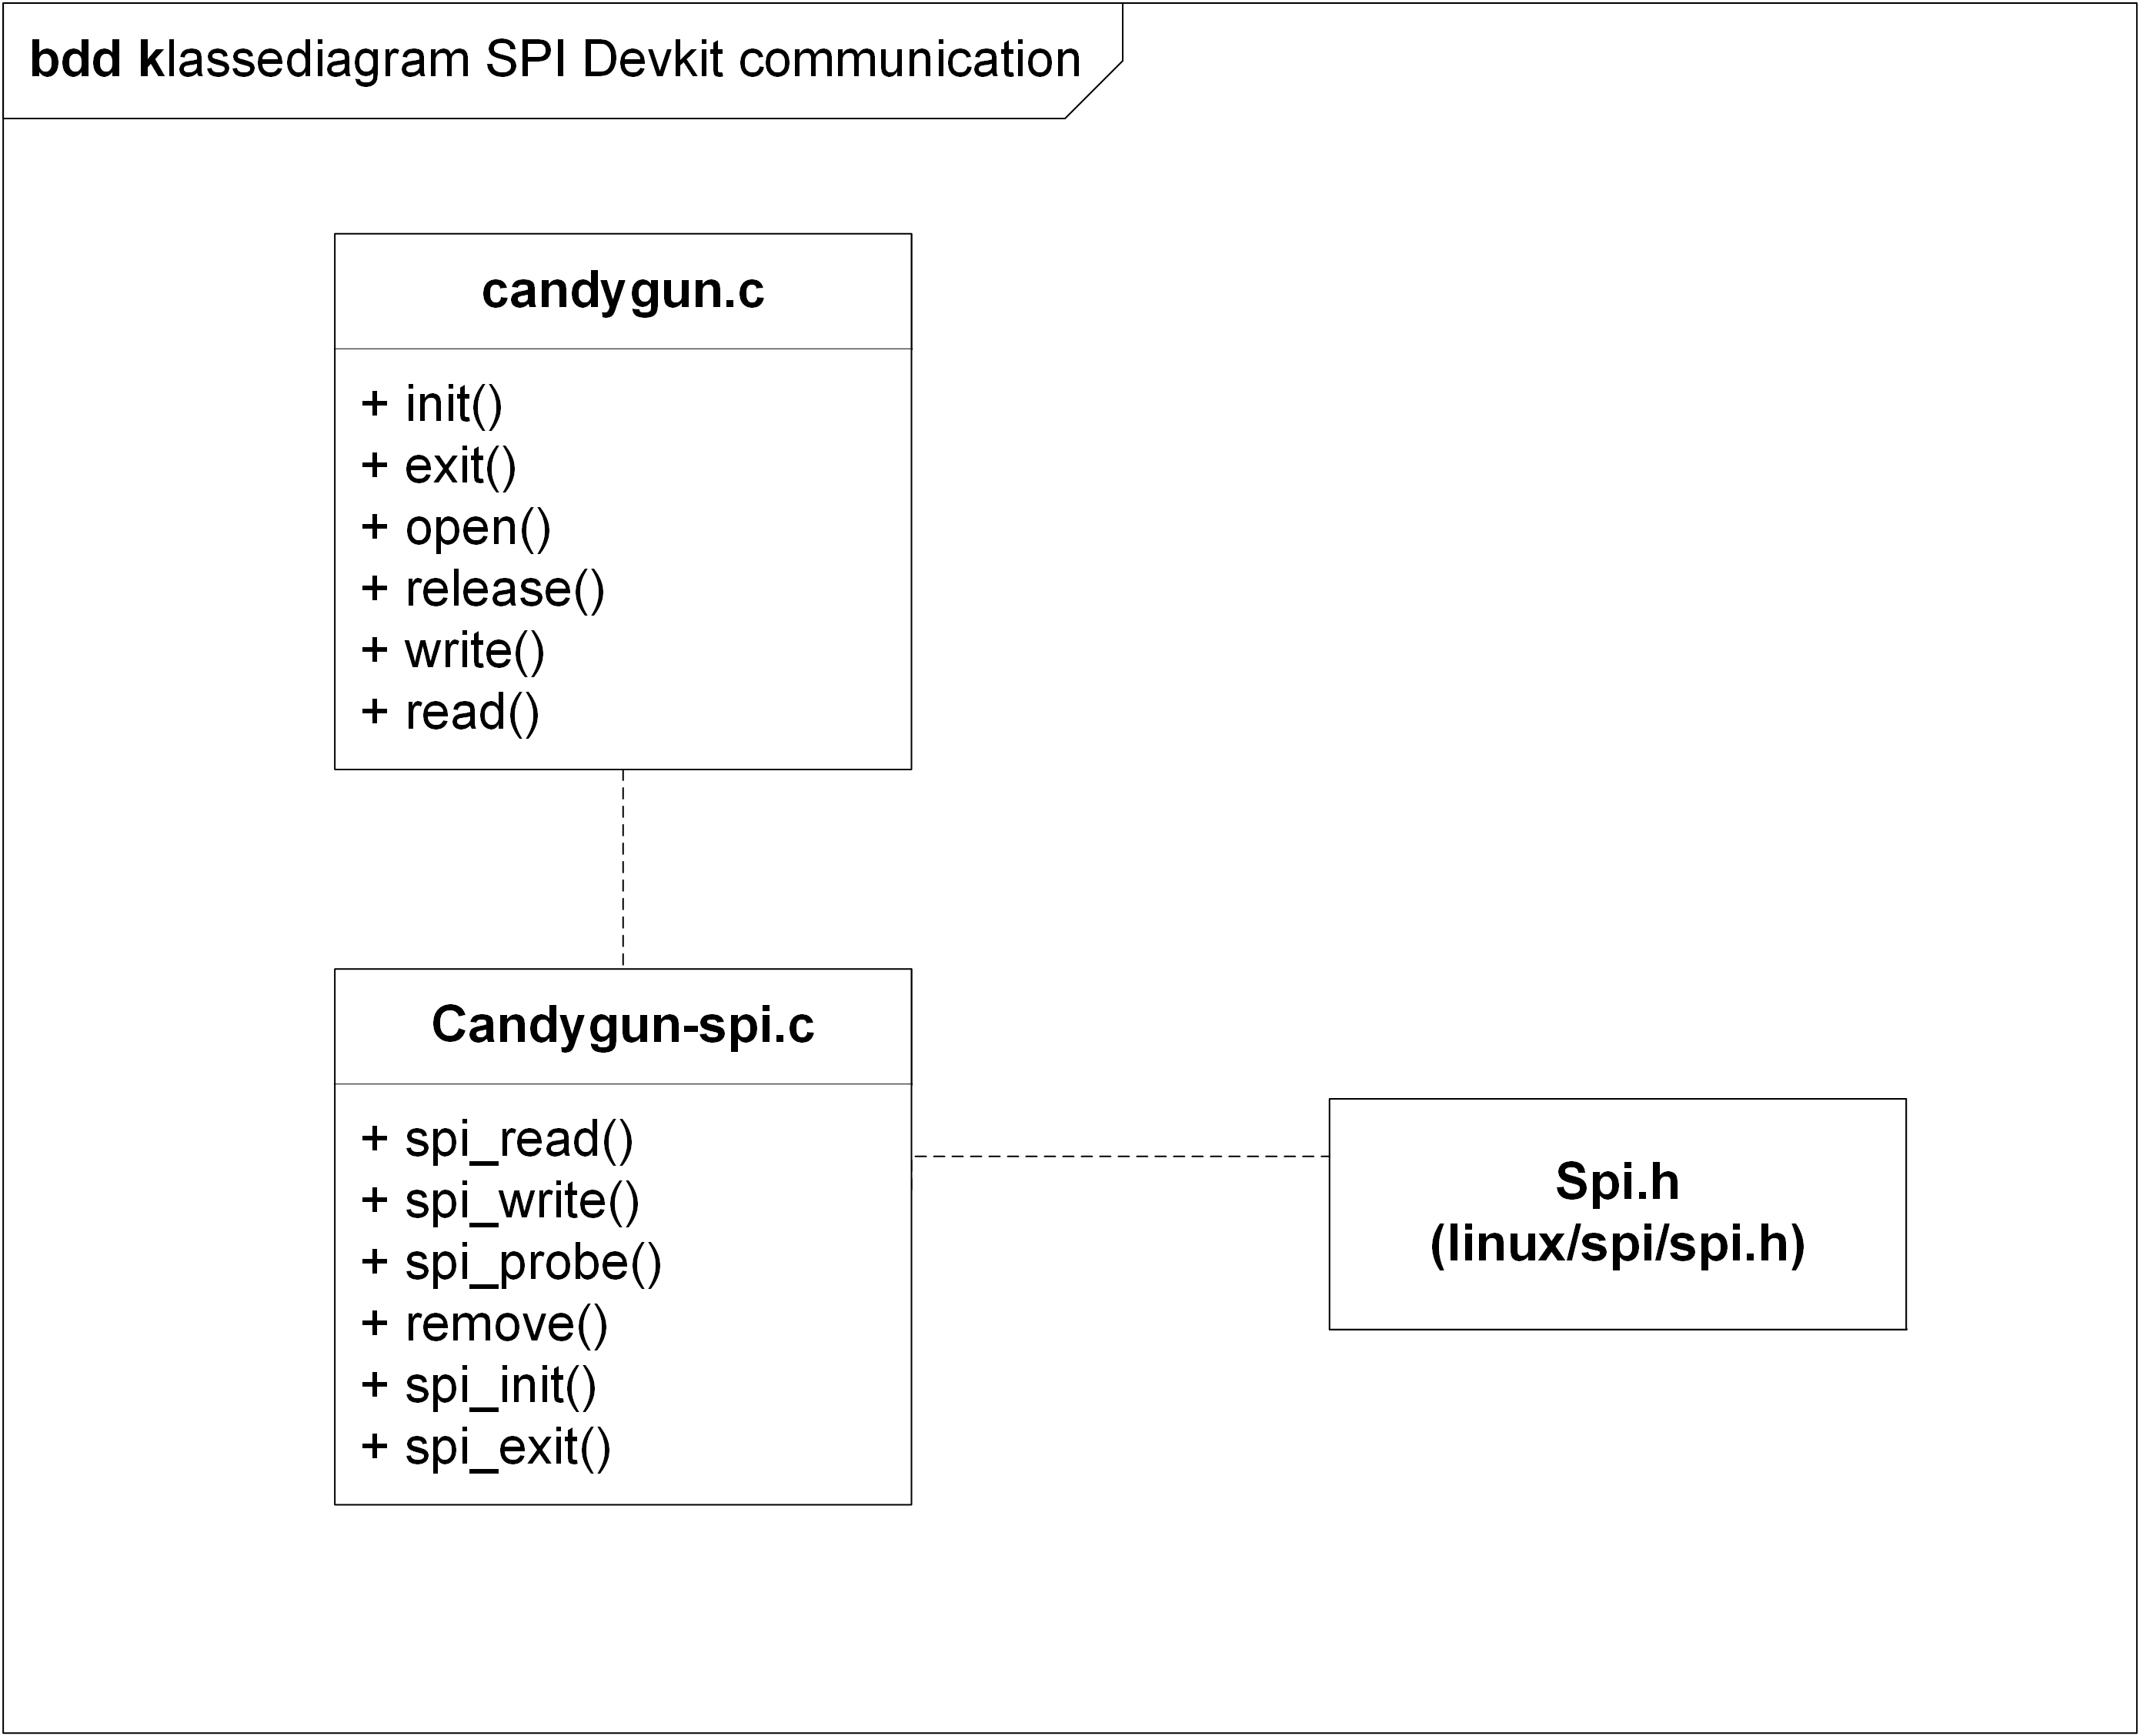
\includegraphics[width=\textwidth]{Afsnit/DesignOgImplementering/images/SPIklasse}
 	\caption{Klassediagram for SPI kommunikation på Devkit 8000}
 	\label{fig:spiklasse}
 \end{figure}
 
\subsubsection{Opbygning af write-metode}
I write-metoden gives der data med fra brugeren. I dette tilfælde udgøres brugeren af Interface driveren og dataet er en 8 bit kommando fra SPI-protokollen. Dog er dataet fra brugeren i første omgang læst ind som en charstreng. I write-metoden bliver det så lavet om til en int.  For at overføre dataet på en sikker måde anvendes funktionen copy\textunderscore from\textunderscore user() til at overføre data fra brugeren. Write-funktionen fra candygun.c anvender derefter en write-funktion fra candygun-spi.c, hvor den sender brugerinputtet med. I den spi-relaterede write-funktion bliver bruger inputtet lagt i transfer bufferen og der NULL bliver lagt i receive bufferen, og med spi\textunderscore sync-funktionen bliver det sendt. På figur \ref{fig:spiwrite} ses et sekvensdiagram for writemetoden, med fokus på opbygningen af den besked, der skal sendes.\\

 \begin{figure}[H]
 	\centering 
 	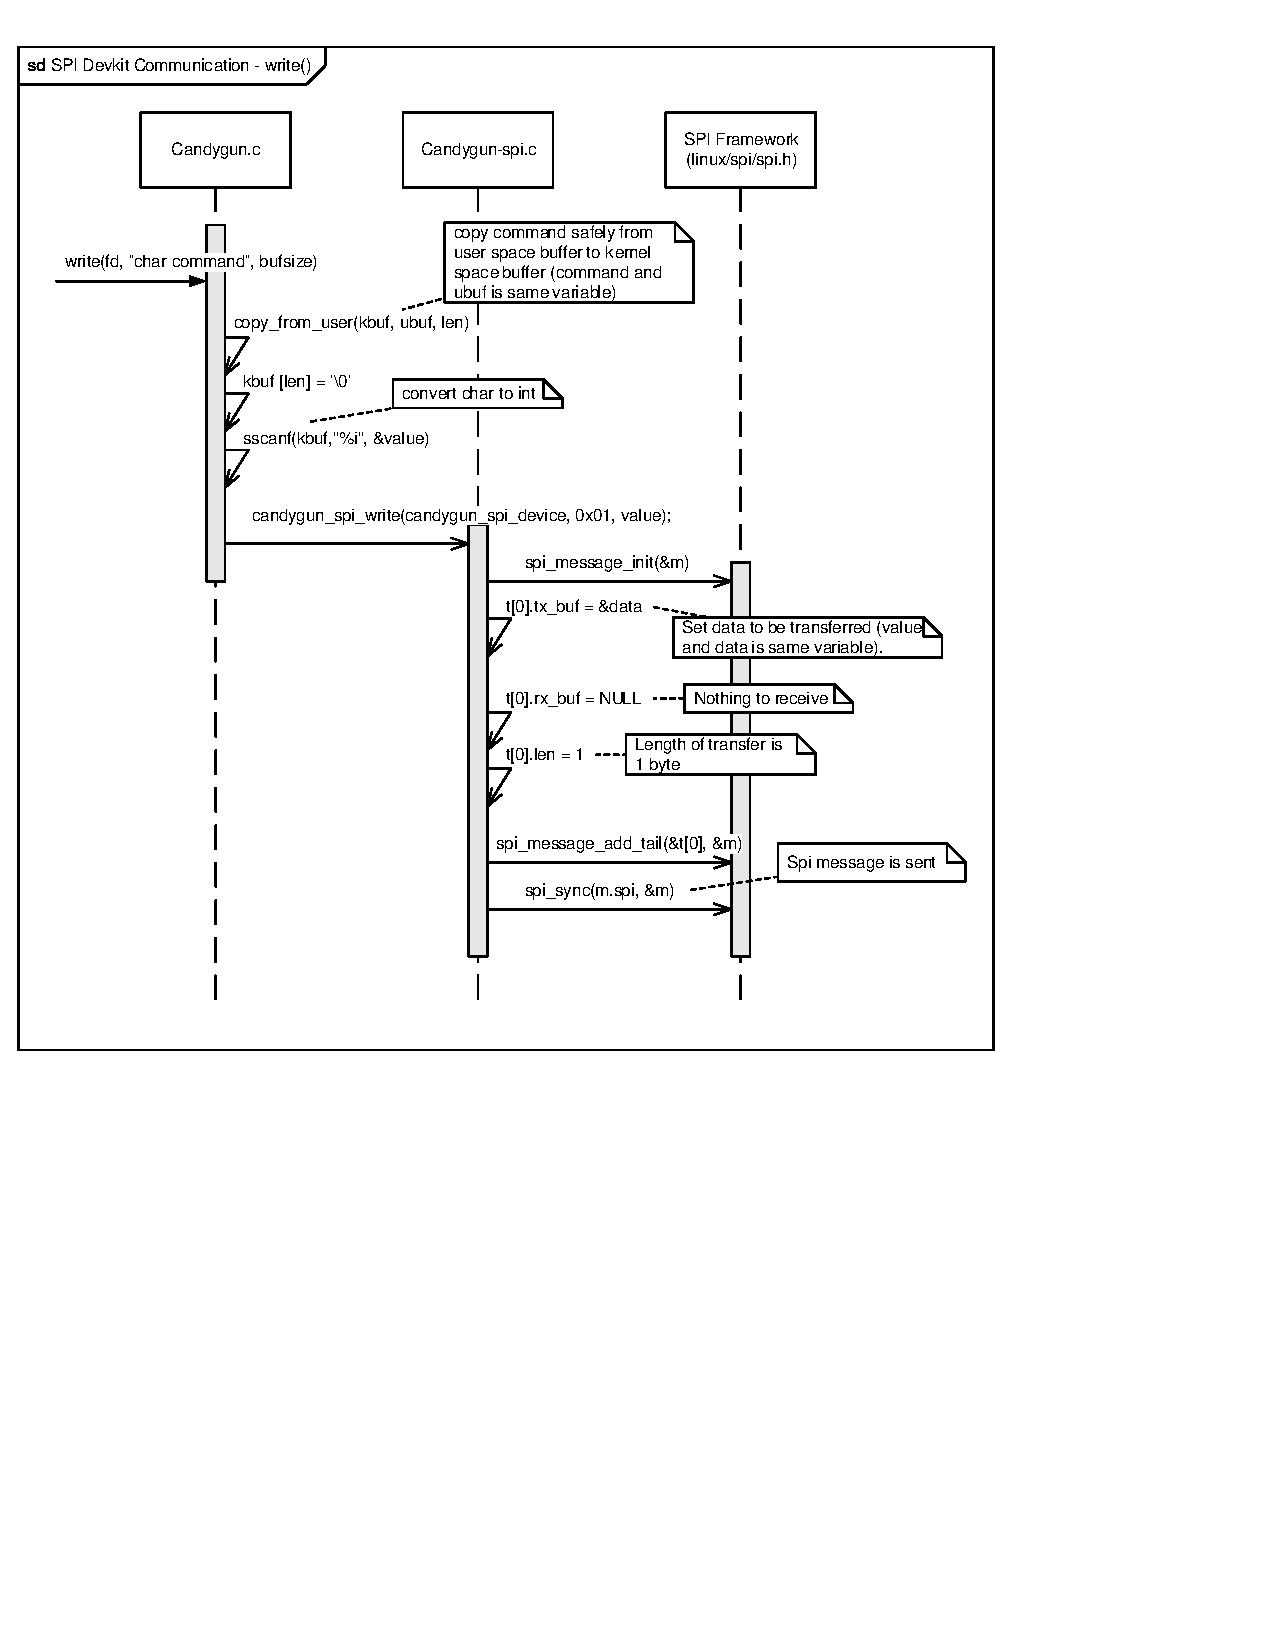
\includegraphics[width=1.25\textwidth, trim = {0 10cm 0 0}]{Afsnit/DesignOgImplementering/images/SPIsekvenscom}
 	\caption{Sekvensdiagram for SPI write kommunikation på Devkit 8000}
 	\label{fig:spiwrite}
 \end{figure}

\subsubsection{Opbygning af read-metode} 
Ofte ville der en spi read-funktion først indeholde en write-del, som fortæller SPI-slaven, hvad der skal læses over i bufferen. Det ville typisk efterfølges af et delay og så en read-del. Men i dette projekt skal der ofte afventes et brugerinput, som ikke kan styres af et fast delay, og der skal generelt sendes en aktiv kommando før der læses. Derfor er det besluttet at read-funktionen kun indeholde en read-del i transmissionen. Dermed skal write-funktionen altid aktivt anvendes inden der læses, da PSoC0 ellers ikke ved, hvad der skal gøres/lægges i bufferen.
Når funktionen har modtaget resultatet fra transmissionen returneres det til brugeren med funktionen copy\textunderscore to\textunderscore user(), som igen sørger for at overførslen af data foregår på en sikker måde.
Et sekvensdiagram for read-funktionen ses på figur \ref{fig:spiread}. Igen er hovedformålet at forklare, hvordan en SPI-message er opbygget i denne driver.\\

 \begin{figure}[H]
 	\centering 
 	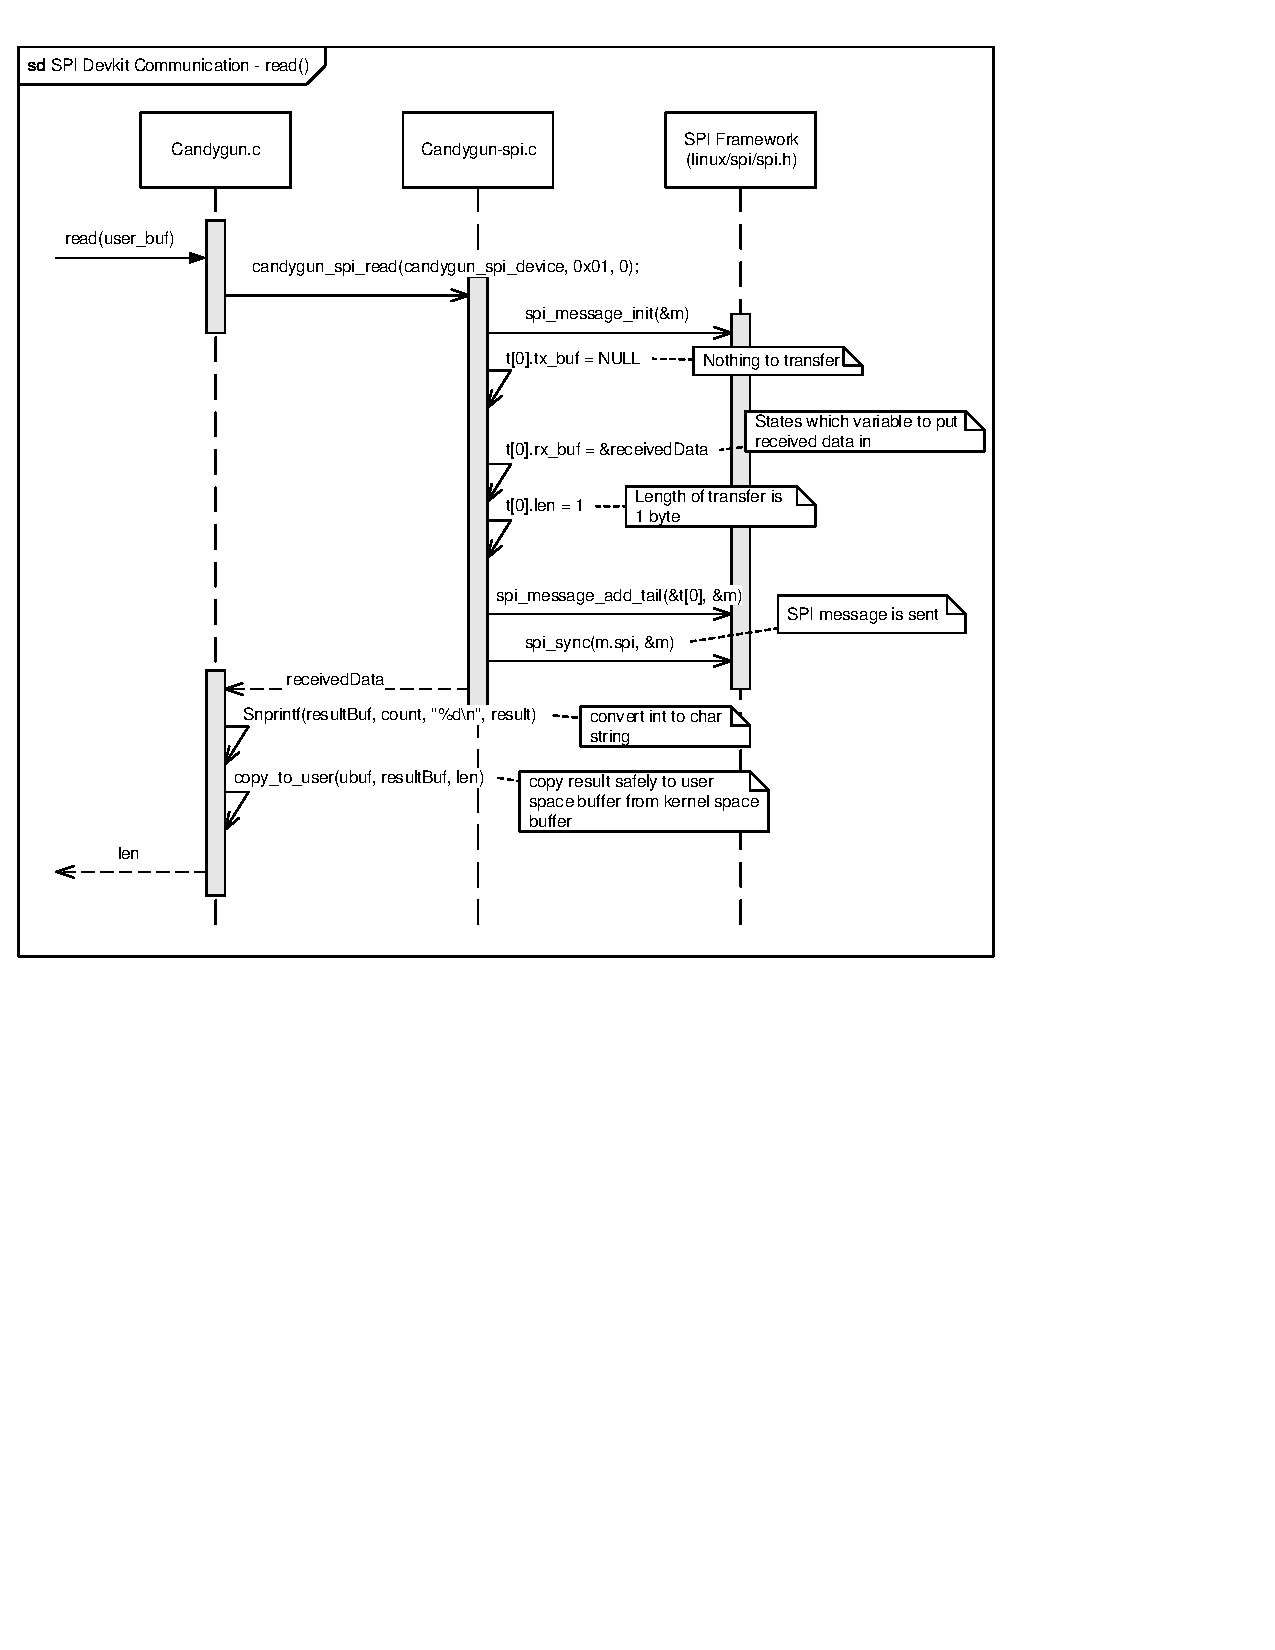
\includegraphics[width=1.25\textwidth, trim = {0 11.6cm 0 0}]{Afsnit/DesignOgImplementering/images/SPIsekvensRead}
 	\caption{Sekvensdiagram for SPI read kommunikation på Devkit 8000}
 	\label{fig:spiread}
 \end{figure}

\subsubsection{Hotplug}
For at kunne anvende driveren, når SPI er tilsluttet, er der oprettet et hotplugmodul, som fortæller kernen, at der er et SPI device, som matcher driveren. Det kan SPI-forbindelsen ikke selv gøre, som usb fx kan.

\subsubsection{Metodebeskrivelser}

\textit{\textbf{candygun.c:}} \\

\noindent\textbf{static int \_\_init candygun\_cdrv\_init(void)} \\
I initfunktionen bliver devicenumre allokeret dynamisk, og kernen informeres om cdev-strukturen. Desuden anvendes candygun\_spi\_init() fra candygun-spi.c til at requeste en spi ressource. \\

\noindent\textbf{static void \_\_exit candygun\_cdrv\_exit(void)}\\
Afregistrer device og klasse fra kernen. Anvender candygun\_spi\_exit() fra candygun-spi.c til at frigive SPI-ressource.\\

\noindent\textbf{int candygun\_cdrv\_open(struct inode *inode, struct file *filep)} \\
Kaldes når det kernemodul, der skal skrives til for at anvende driveren, åbnes. Tjekker om device-numrene passer. Printer en kernebesked om at modulet åbnes.\\

\noindent\textbf{int candygun\_cdrv\_release(struct inode *inode, struct file *filep)} \\
Kaldes når kernemodulet lukkes. Printer en kernebesked om at modulet lukkes.\\
 
\noindent\textbf{ssize\_t candygun\_cdrv\_write(struct file *filep, const char \_\_user *ubuf, size\_t count, loff\_t *f\_pos)} \\
Sørger for at klargøre en kommando fra userspace, og giver den med til funktionen candygun\_spi\_write(), som håndterer SPI-kommunikationen.\\

\noindent\textbf{ssize\_t candygun\_cdrv\_read(struct file *filep, char \_\_user *ubuf, size\_t count, loff\_t *f\_pos)}
Anvender candygun\_spi\_read(), som håndtere læsning ved SPI. Sørger derefter for at omdanne returværdien til en string og copiere den sikkert til userspace. \\

\noindent\textit{\textbf{candygun-spi.c}} \\

\noindent\textbf{int candygun\_spi\_init(void)} \\
Requester en SPI-ressouce. \\

\noindent\textbf{void candygun\_spi\_exit(void)} \\
Frigiver SPI-ressource. \\

\noindent\textbf{static int candygun\_spi\_probe(struct spi\_device *spi)} \\
Probe køres når driveren bliver "insmod"'et i kernen, for at se om der er et SPI-device, der matcher modalias for driveren.\\

\noindent\textbf{static int candygun\_remove(struct spi\_device *spi)} \\ 
Fjerner SPI-device på chip-select.\\

\noindent\textbf{int candygun\_spi\_write(struct spi\_device *spi, u8 addr, u8 data)} \\
Håndterer opbyggelsen af en SPI-message, sætter receivebufferen til NULL, da der ikke skal læses, og anvender funktioner fra linux/spi/spi.h til at udføre SPI-transfer. \\

\noindent\textbf{int candygun\_spi\_read(struct spi\_device *spi, u8* value)} \\
Håndterer opbyggelsen af en SPI-message, sætter transferbufferen til NULL, da der ikke skal skrives, sætter en kerne buffer til receive, og anvender funktioner fra linux/spi/spi.h til at udføre SPI-transfer.  \\


\subsection{Brugergrænseflade}
I dette afsnit beskrives de forskellige dele af brugergrænsefladen.

\subsubsection{Interfacedriver}
Interface driveren er bindeled mellem brugergrænsefladen og candydriveren. Interface driveren er implementeret i c++. Den indeholder fire funktioner til use case 2. De håndterer test af de forskellige kommunikationsforbindelser i systemet. Candygun klassen implementerer de rigtig funktioner med forbindelse til det restende system, og anvender de nødvendige funktioner til at skrive til og læse fra et kernemodul. På figur \ref{fig:InterfacedriverKlassediagram} ses klassediagrammet for Interface Driveren. 

\begin{figure}[H]
	\centering
	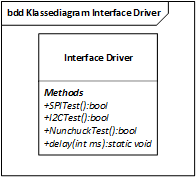
\includegraphics[width=\textwidth]{DesignOgImplementering/images/InterfacedriverKlassediagram}
	\caption{Klassediagram for Interface driveren på Devkit8000}
	\label{fig:InterfacedriverKlassediagram}
\end{figure}

\paragraph{Klassebeskrivelse} \mbox{} \\

bool SPITest():
Denne metode initierer SPI-test ved at skrive SPI-kommandoen "241" til "dev/candygun", som er den node, der oprettes af Candydriveren. Dernæst indeholder funktionen et delay på 1 sek, for at give SPI-testen tid til at blive udført. Til sidst læser funktionen fra "dev/candygun" og tjekker om den får den korrekte returværdi, "209". Ved korrekt returværdi returnerer funktionen true. Ved fejl returnerer funktionen false.      

bool I2CTest():
Denne metode initierer I2C-test ved at skrive I2C-kommandoen "242" til "dev/candygun", som er den node, der oprettes af Candydriveren. Dernæst indeholder funktionen et delay på 1 sek, for at give I2C-testen tid til at blive udført. Til sidst læser funktionen fra "dev/candygun" og tjekker om den får den korrekte returværdi, "210". Ved korrekt returværdi returnerer funktionen true. Ved fejl returnerer funktionen false.

bool nunchuckTest():	
Denne metode initierer nunchuck-test ved at skrive nunchuck-kommandoen "251" til "dev/candygun", som er den node, der oprettes af Candydriveren. Metoden tjekker "dev/candygun" efter 6 sekunder, om der er trykket på nunchuckknappen. Det ses ved den korrekte returværdi, "211". Ved korrekt returværdi returnerer funktionen true.

static void delay(int ms):
Denne metode initierer et delay. Det valgte antal ms bliver lagt til det interne systemur. Når systemuret når til det sammenlagte tidspunkt, fortsættes programmet.

\subsubsection{Systemtest GUI}
Usecase 2 styres via Systemtest GUI'en fra Devkit8000.
Dette afsnit beskriver Systemtest GUI'ens design.

\begin{figure}[H]
	\centering
	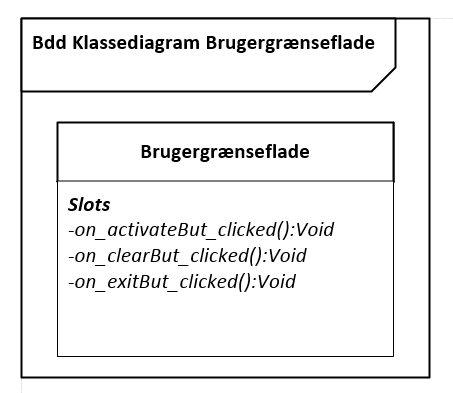
\includegraphics[width=\textwidth]{DesignOgImplementering/images/KlassediagramGUI}
	\caption{Klassediagram for Systemtest GUI}
	\label{fig:KlassediagramGUI}
\end{figure}

\paragraph{Klassebeskrivelse}\mbox{} \\
\label{sec:stmDescrip}

\noindent void on\_activateBut\_clicked(): \newline
Dette slot er startknappen i brugergrænsefladen. Ved tryk bliver knappens signal broadcastet og knappens funktion bliver kørt. Forløbet for dette slot beskrives i figur \ref{fig:stmGUI}. Der skrives til konsolvinduet, derefter testes der på SPITest(). Hvis der returnes true, skrives dette til konsollen og programmet fortsætter til I2CTest(). Hvis der returnes false, skrives dette til konsollen og programmet returnerer til idle-tilstand. Nu testes der på I2CTest(). Hvis der returnes true, skrives dette til konsollen og programmet fortsætter til NunchuckTest(). Hvis der returnes false, skrives dette til konsollen og programmet returnerer til idle-tilstand.
Der testes der på NunchuckTest(). Hvis der returnes true, skrives dette til konsollen, og der skrives at systemtesten er gennemført. Hvis der returnes false, skrives dette til konsollen. Programmeret returnerer til idle-tilstand. \newline

\noindent void on\_clearBut\_clicked(): \newline
Dette slot er clearknappen i brugergrænsefladen. Knappens funktionalitet er en clearing af konsol vinduet. \newline

\noindent void on\_exitBut\_clicked(): \newline
Dette slot er exitknappen i brugergrænsefladen. Knappens funktionalitet består i, at programmet lukkes.


\begin{figure}[H]
	\centering
	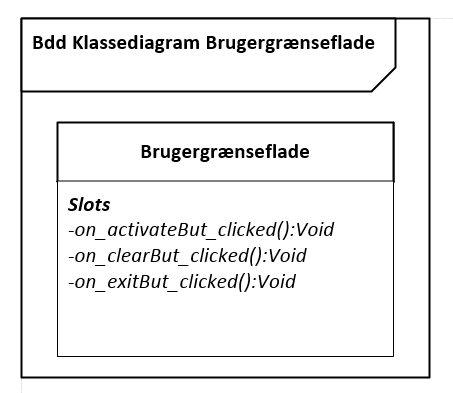
\includegraphics[width=\textwidth]{DesignOgImplementering/images/KlassediagramGUI}
	\caption{Statemachine for Systemtest GUI}
	\label{fig:stmGUI}
\end{figure}

\subsubsection{Demo GUI}
I dette afsnit beskriver Demo GUI'en for usecase 1.
Strukturen for denne GUI er lignende til Systemtest GUI'en.
Denne demo er en repræsentation af hvad der kunne være en færdig implementeret GUI til usecase 1.

\begin{figure}[H]
	\centering
	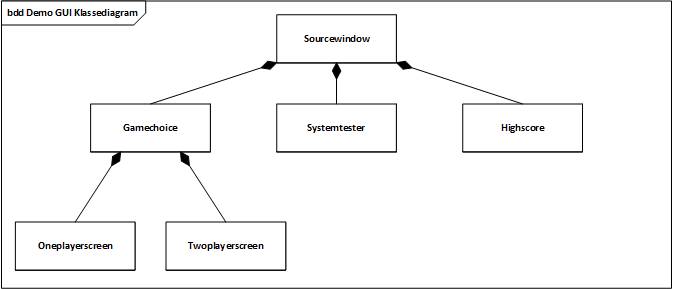
\includegraphics[width=1.2\textwidth]{Afsnit/DesignOgImplementering/images/DemoGUIClass}
	\caption{Klassediagram for Demo GUI}
	\label{fig:DemoGUIClass}
\end{figure}

\paragraph{Klassebeskrivelse} \mbox{} \\

\label{afsnit:democlass}

\noindent\textbf{Sourcewindow:}\newline
Klassens vindue består af fire knapper med følgende\newline
\noindent \textbf{Slots:}\newline
void on\_exitBut\_clicked():\newline
Denne knap har den samme funktion som exitBut fra metodebeskrivelsen afsnit \#ref \newline

\noindent void on\_scoreBut\_clicked():\newline
Denne knap åbner vinduet til Highscore-klassen.\newline

\noindent void on\_startBut\_clicked():\newline
Denne knap åbner vinduet til Gamechoice-klassen.\newline

\noindent void on\_testBut\_clicked():\newline
Denne knap åbner vinduet til Systemtester-klassen, se afsnit for \#Systemtestgui for beskrivelse.\newline

\noindent\textbf{Highscore:}\newline
Klassens vindue består af et konsol vindue og tre knapper med følgende\newline
\noindent \textbf{Slots:}\newline
\noindent void on\_setHiBut\_clicked():\newline
Denne knap skriver nogle testværdier til konsol vinduet.\newline

\noindent void on\_clearHiBut\_clicked():\newline
Denne knap clearer konsol vinduet. \newline

\noindent void on\_exitHiBut\_clicked();\newline
Denne knap lukker Highscore vinduet og GUI'en returnerer til sourcewindow.\newline

\noindent\textbf{Gamechoice:}\newline
\noindent Klassens vindue består af tre knapper med følgende \newline
\noindent \textbf{Slots:}\newline
\noindent void on\_choiceOne\_clicked():\newline
Denne knap åbner vinduet til Oneplayerscreen-klassen, og
den opretter et oneplayerscreen objekt og kalder en slot-funktionen setTestScores fra oneplayerscreen.\newline

\noindent void on\_choiceTwo\_clicked():\newline
Denne knap åbner vinduet til Twoplayerscreen-klassen, og
den opretter et twoplayerscreen objekt og kalder en slot-funktionen setTestScores fra twoplayerscreen.\newline

\noindent void on\_choiceExitBut\_clicked():\newline
Denne knap lukker Gamechoice vinduet og GUI'en returnerer til sourcewindow.\newline

\noindent\textbf{Oneplayerscreen:}\newline
Klassens vindue består af et konsol vindue, en knap med følgende\newline
\noindent \textbf{Slots:}\newline
void on\_playerExitBut\_clicked():\newline
Denne knap lukker Oneplayerscreen vinduet og GUI'en returnerer til Gamechoice.\newline

\noindent void setTestScores():\newline
Dette slot skriver testværdier til Oneplayerscreen's konsol vindue.\newline

\noindent \textbf{Twoplayerscreen:}\newline
Klassens vindue består af to konsol vinduer, en knap med følgende\newline
\noindent \textbf{Slots:}\newline
void on\_twoExitBut\_clicked():\newline
Denne knap lukker Twoplayerscreen vinduet og GUI'en returnerer til Gamechoice.\newline

\noindent void setTestScores():\newline
Dette slot skriver testværdier til Twoplayerscreen's konsol vinduer.

\begin{figure}[H]
	\centering
	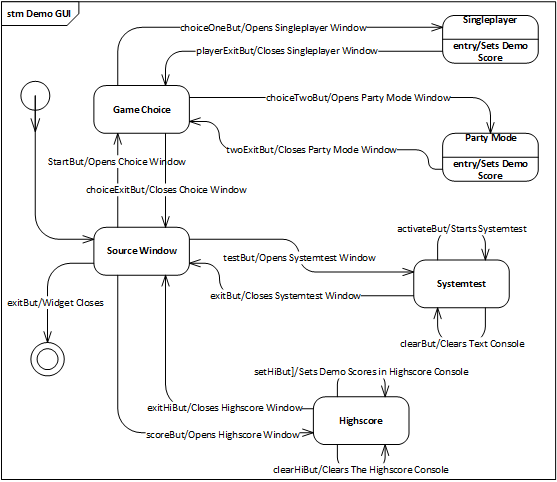
\includegraphics[width=1.2\textwidth]{Afsnit/DesignOgImplementering/images/StateMachineDemoGUI}
	\caption{State machine for Demo GUI}
	\label{fig:StateMachineDemo}
\end{figure}

Denne State Machine giver en visuel repræsentation af skiften mellem GUI-vinduer.  Hvert knaptryk er et event og slot-funktionen for den pågældende knap bliver kørt.
Se klassebeskrivelsen,\ref{afsnit:democlass} for detaljeret beskrivelse.

\section{PSoC Software}
På figur \ref{figure:klassediagramPSoC0} og \ref{figure:klassediagramPSoC1} ses de endelige klassediagrammer for PSoC0 og PSoC1. Disse klassediagrammer er designet ud fra applikationsmodellerne for use case 1 og 2 i afsnit \ref{afsnit:applikationsmodelUC1} og \ref{afsnit:applikationsmodelUC2}, samt de samlede klassediagrammer for use case 1 og 2 i systemarkitekturen afsnit \ref{afsnit:samledeKlassediagrammer} figur \ref{fig:CompleteClassDiagramPSoC0} og \ref{fig:CompleteClassDiagramPSoC1}. For at opretholde høj samhørighed, er der lavet en klasse for hver grænseflade. Dette kan ses på figur \ref{figure:klassediagramPSoC0}, da separate klasser er oprettet for grænsefladerne \textit{SPI}, \textit{I2C}, samt \textit{Nunchuck} controlleren. De efterfølgende afsnit vil beskrive klasserne og deres funktioner.

\begin{figure}[H]
	\begin{adjustwidth}{-2cm}{-\rightmargin}
		\centering
		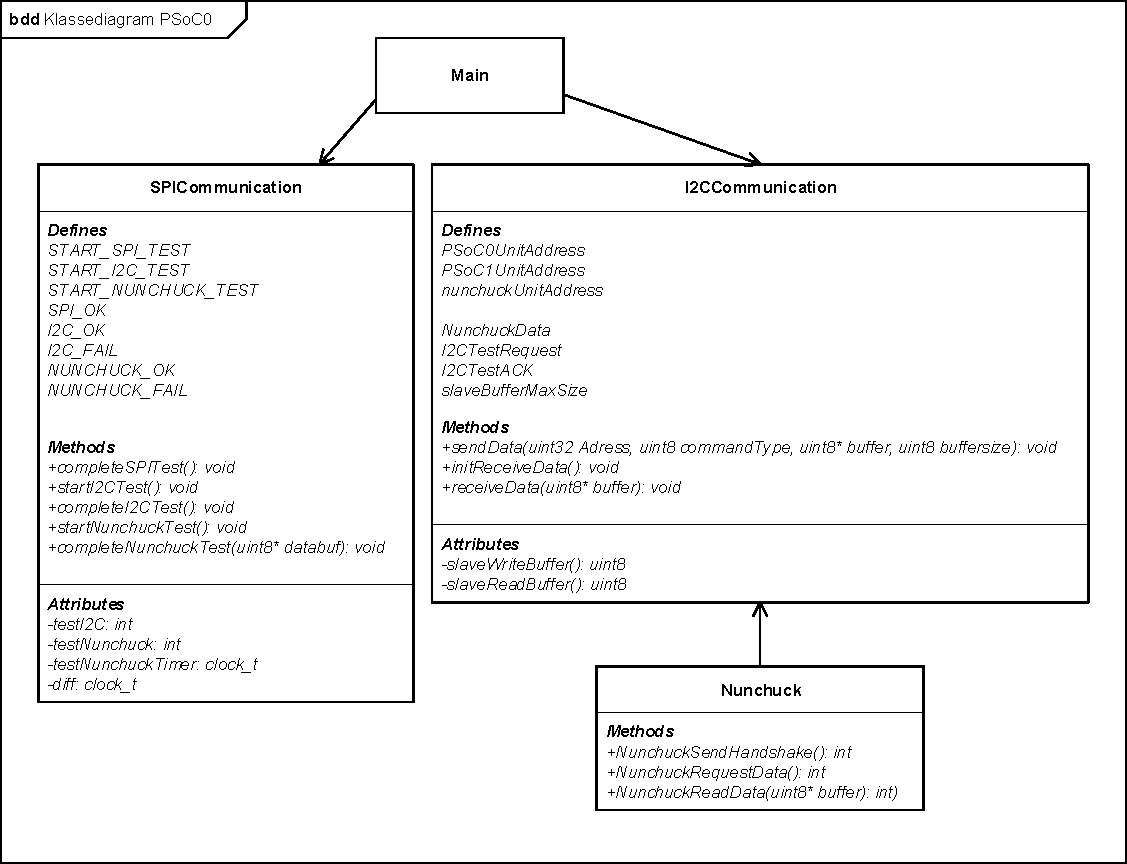
\includegraphics[width=1.35\textwidth]{DesignOgImplementering/images/PSoC0KlassediagramOversigt.pdf}
		\caption{Klassediagram for PSoC0}
		\label{figure:klassediagramPSoC0}
	\end{adjustwidth}
\end{figure}

På figur \ref{figure:klassediagramPSoC0} ses det samlede klassediagram for klasserne som bruges til PSoC0 softwaren. Her kan det ses at der er en \textit{main} klasse. Denne indeholder programmets primære loop, som gentages indtil PSoC'en slukkes. I dette loop bliver der gjort brug af funktionaliteten fra klasserne \textit{SPICommunication}, \textit{I2CCommunication}, samt \textit{Nunchuck}. Disse klasser beskrives i afsnit \ref{afsnit:SPIcommunication}, \ref{afsnit:I2Ccommunication} og \ref{afsnit:nunchuckDI}.

\begin{figure}[H]
	\centering
	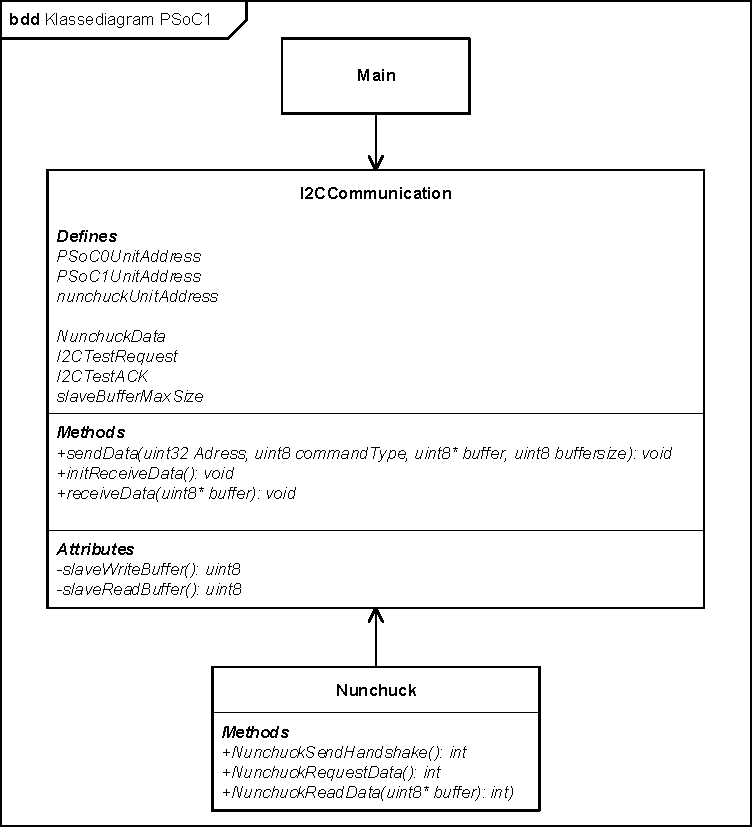
\includegraphics[width=\textwidth]{DesignOgImplementering/images/PSoC1KlassediagramOversigt.pdf}
	\caption{Klassediagram for PSoC1}
	\label{figure:klassediagramPSoC1}
\end{figure}

På figur \ref{figure:klassediagramPSoC1} ses det samlede klassediagram for klasserne som eksisterer på PSoC1 softwaren. Her kan det ses at der er en \textit{main} klasse. Denne indeholder programmets primære loop, som gentages indtil PSoC'en slukkes. I dette loop bliver der gjort brug af funktionaliteten fra klasserne \textit{I2CCommunication} og \textit{Nunchuck}. Disse klasser beskrives ligeledes i afsnit \ref{afsnit:SPIcommunication} og \ref{afsnit:I2Ccommunication}.

\subsection{SPICommunication}
\label{afsnit:SPIcommunication}
I dette afsnit vil softwaren der specifikt omhandler SPI kommunikationen mellem PSoC0 og Devkit 8000 blive beskrevet. Dette gøres med et klassediagram og klassebeskrivelser.

\subsubsection{Klassediagram}
På figur \ref{figure:KlassediagramSPICommunication} ses klassediagrammet over SPICommunication klassen.

\begin{figure}[H]
	\centering
	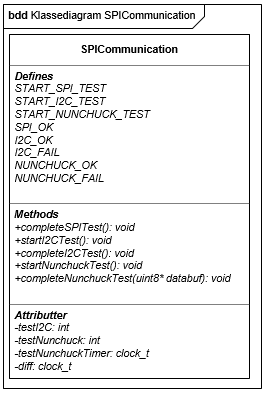
\includegraphics[]{DesignOgImplementering/images/SPICommunication}
	\caption{Klassediagram over SPICommunication}
	\label{figure:KlassediagramSPICommunication}
\end{figure}

\subsubsection{Klassebeskrivelser}
Klassen \textit{SPICommunication} har til ansvar at gennemføre SPI-, I2C-, samt Nunchucktesten som bliver anmodet om af Devkit 8000 under use case 2. Dette gøres ved nedenstående metoder. \newline

\noindent\textbf{void completeSPITest()} \newline
Denne metode gemmer \textit{SPI\_OK} i PSoC'ens SPI-transfer buffer. \newline

\noindent\textbf{void completeI2CTest()} \newline
Denne metode gennemfører I2C-Testen. Dette gøres ved at der sendes en besked til alle enheder på I2C-nettet, og hvis der ikke registreres nogen fejl på denne besked, bliver \textit{I2C\_OK} gemt i PSoC'ens SPI-transfer buffer. Registreres der en fejl, bliver \textit{I2C\_FAIL} gemt i SPI-transfer buffer. \newline

\noindent\textbf{void completeNunchuckTest(uint8* databuf)} \newline
\noindent Denne metode gennemfører Nunchuck-testen. Dette gøres ved at der startes en timer på 5 sekunder. Hvis der sker et tryk på 'Z'-knappen på nunchucken indenfor disse 5 sekunder, vil \textit{NUNCHUCK\_OK} blive gemt i SPI-transfer bufferen. Hvis der ikke registreres nogen tryk inden for de 5 sekunder, er det \textit{NUNCHUCK\_FAIL} der gemmes.\newline

\noindent I klassediagrammet er der beskrevet en række "Defines". Disse defines bruges i klassen som unikke ID'er der indikerer om en test er gennemført OK eller om den er fejlet.

\subsubsection{SPI Indstillinger på PSoC}
I forbindelse med SPI bussen skal der sættes nogle indstillinger på PSoC0, idét at denne kommunikerer med Devkit 8000 via SPI. 
PSoC'en sættes til slave, idét at det er Devkit 8000 der aflæser og skriver til PSoC0.
SCLK sættes til CPHA=1 og CPOL=1. Disse er valgt arbitrært, dog ud fra den forudsætning, at de skal stemme overens med indstillingerne på Devkit 8000, idét disse indstillinger beskriver hvornår databit aflæses eller sættes i forhold til clock'en. 
\textit{Data Rate} sættes til 1Mbps, da dette er en stabil overførselshastighed. Denne indstilling skal være ens for PSoC og Devkit 8000. Den sidste indstilling der sættes, er \textit{transfer} og \textit{read} buffer size. Disse er valgt til at være 8-bit, da projektets SPI kommunikationsprotokol ikke har brug for størrer datamængder. Denne indstilling skal være ens for både SPI master og SPI slave.

\subsubsection{Test Opstart Algoritme}
På figur \ref{figure:TestStartAlgorithm} ses et aktivitetsdiagram for algoritmen som eksekverer de forskellige tests afhængig af den modtagne kommandotype fra Devkit 8000.

\begin{figure}[H]
	\centering
	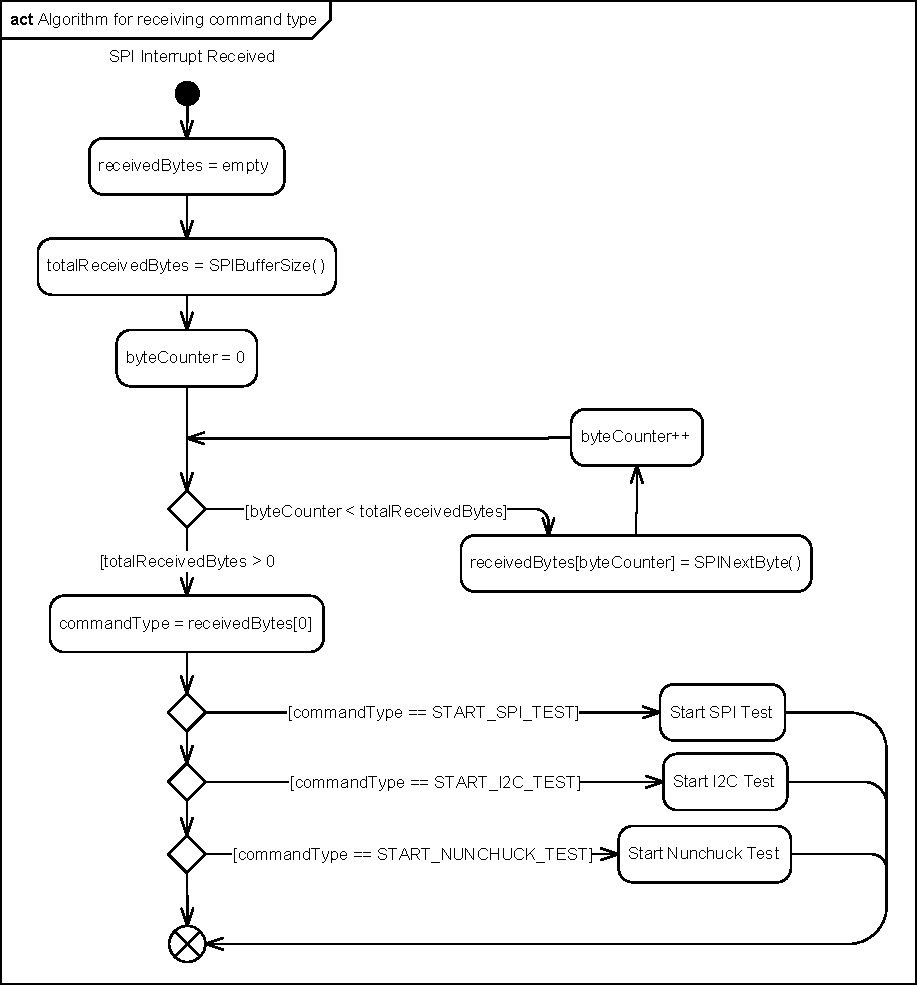
\includegraphics[width=\textwidth]{DesignOgImplementering/images/SPITestActivity}
	\caption{Aktivitetsdiagram der viser algoritmen som bestemmer hvilket test der skal eksekveres}
	\label{figure:TestStartAlgorithm}
\end{figure}

\noindent På tabel \ref{table:SPIActivityVariables} ses en forklaring af de variable der indgår i algoritmen.

\begin{table}[H]
	\centering
	\begin{tabular}{|l|l|}
		\hline
		Variable         & Beskrivelse                                                                                                                                              \\ \hline
		receivedBytes    & \begin{tabular}[c]{@{}l@{}}Denne variabel er et array som \\ indeholder modtagede bytes fra SPI bussen. \end{tabular}                              \\ \hline
		totalReceivedBytes & \begin{tabular}[c]{@{}l@{}}Denne variabel indeholder antallet \\ af modtagede bytes fra SPI bussen.\end{tabular} \\ \hline
		byteCounter & \begin{tabular}[c]{@{}l@{}}Denne variabel er en tæller \\  til algoritmens for løkke.\end{tabular} \\ \hline
		commandType & \begin{tabular}[c]{@{}l@{}}Denne variabel indeholder kommandotypen \\ af den modtagede kommando.\end{tabular} \\ \hline
	\end{tabular}
	\caption{Variable der indgår i aktivitetsdiagrammet figur \ref{figure:TestStartAlgorithm}}
	\label{table:SPIActivityVariables}
\end{table}

\noindent Aktivitetsdiagrammet, figur \ref{figure:TestStartAlgorithm}, viser at algoritmen bliver eksekveret hver gang et SPI interrupt modtages. Et SPI interrupt opstår når nyt data fra SPI bussen er modtaget og klart til at blive læst fra bufferen på PSOC'en. Den første betydelige hændelse er at variablen \textit{totalReceivedBytes} bliver sat til antallet af modtagede bytes fra SPI bussen. Herefter køres en for løkke igennem, hvor alle modtagede bytes fra PSOC'ens buffer bliver overført til variablen \textit{receivedBytes}. Til slut tjekkes den første modtagede byte, da denne indeholder kommandotypen modtaget på SPI bussen. Ud fra denne værdi bliver den korrekte test eksekveret.

\subsection{I2CCommunication}
\label{afsnit:I2Ccommunication}
I dette afsnit vil softwaren der omhandler I2C-kommunikation blive beskrevet. Dette inkluderer et klassediagram,  klassebeskrivelser og indstillingerne for I2C kommunikationen på PSoC'en.

\subsubsection{Klassediagram}
På figur \ref{figure:klassediagramI2CCommunication} ses klassediagrammet for I2CCommunication. 
\begin{figure}[H]
	\centering
	%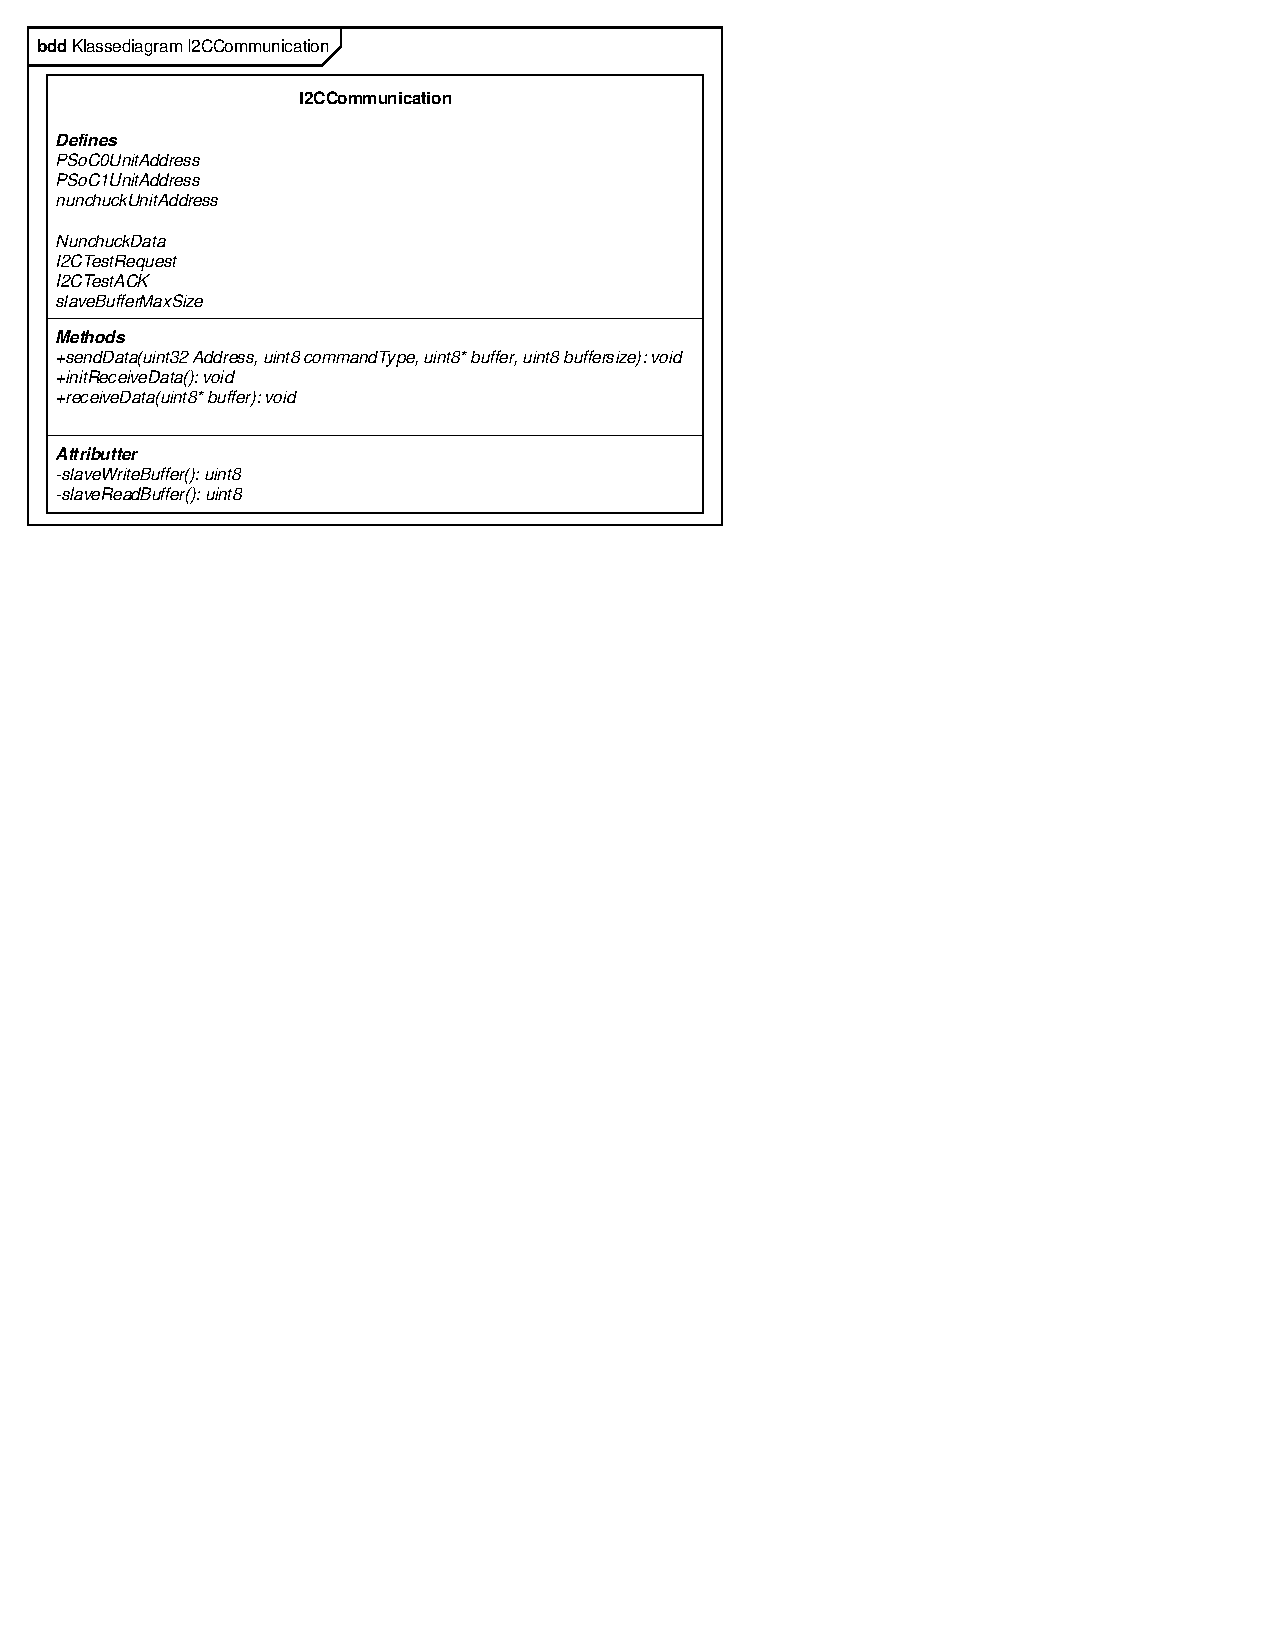
\includegraphics[width=0.9\textwidth, trim={0 19cm 9cm 0},clip]{DesignOgImplementering/images/I2CCommunication.pdf}
	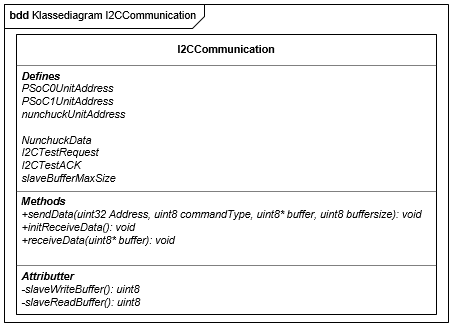
\includegraphics[]{DesignOgImplementering/images/I2CCommunication}
	%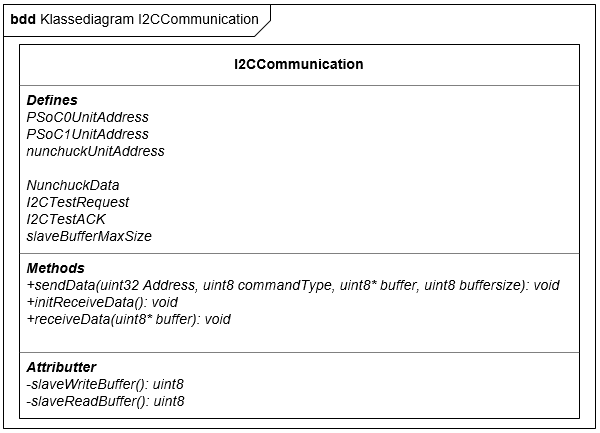
\includegraphics[width =0.9\textwidth]{DesignOgImplementering/images/I2CCommunication2}
	\caption{Klassediagram for I2CCommunication klassen}
	\label{figure:klassediagramI2CCommunication}
\end{figure}

\subsubsection{Klassebeskrivelser}
Som det ses på klassediagrammet figur \ref{figure:klassediagramI2CCommunication} indeholder klassen flere metoder. Disse metoder blive beskrevet her.\newline
\noindent Klassen \textit{I2CCommunication} har til ansvar at skrive og læse data fra I2C bussen. \newline

\noindent\textbf{void sendData(uint8 Address, uint8 commandType, uint8* buffer, uint8 buffersize)}\newline
Denne metode sender, via PSoC Creators I2C-API, den data der ligger i \textit{buffer} af kommandotypen \textit{commandType} til slaven med adressen \textit{Address}. \newline

\noindent\textbf{void initReceiveData()} \newline 
\noindent Denne metode initialiserer de to buffers, \textit{slaveWrite} og \textit{slaveRead}, der kræves på en I2C-slave. Dette gøres ved brug af PSoC Creators I2C-API. \newline

\noindent\textbf{void receiveData(uint8* buffer)}\newline
\noindent Denne metode venter på at slaveRead bufferen er blevet fyldt. Når dette er sket, bliver slaveRead bufferen kopieret over i \textit{buffer}.

\subsubsection{I2C indstillinger på PSoC}
I forbindelse med at have en I2C kommunikation på PSoC'en, er der et par indstillinger der skal sættes. Hver PSoC der gør brug af I2C, sættes til at være en \textit{Multi-master-slave}. Dette gøres for at alle I2C enheder kan gøre brug af \textit{I2CCommunication} klassen, idét at denne indeholder funktioner for både master og slave. 
En anden vigtig indstilling er I2C bussens \textit{Data Rate}. Denne er sat til 100kbps.
Enhver enhed på I2C nettet skal også have en adresse. Adressefordelingen ses i afsnit \ref{afsnit:I2CProtokol} på tabel \ref{table:I2CAddress}.

\subsubsection{Send Data Algoritme}
På figur \ref{figure:SendDataAlgorithm} ses et aktivitetsdiagram for algoritmen der sender databytes ud på I2C bussen.

\begin{figure}[H]
	\centering
	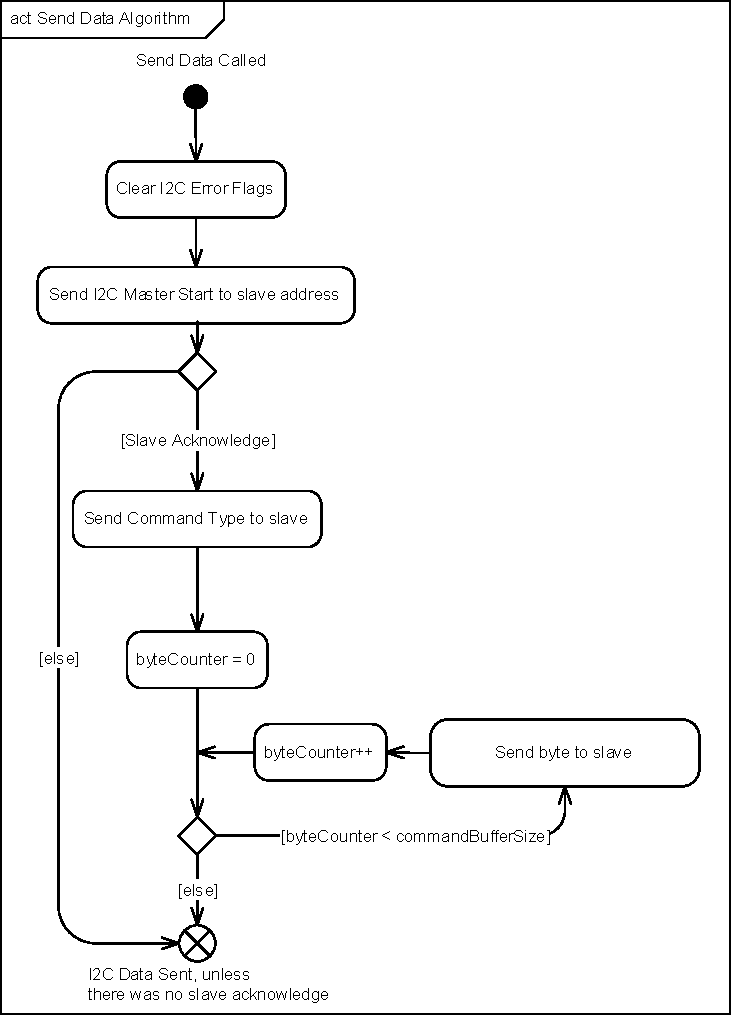
\includegraphics[width=\textwidth]{DesignOgImplementering/images/sendDataAlgorithm}
	\caption{Aktivitetsdiagram over \textit{sendData} metodens algoritme}
	\label{figure:SendDataAlgorithm}
\end{figure}

\noindent Algoritmen starter når funktionen \textit{sendData} bliver eksekveret. Herefter bliver potentielt tidligere fejltilstande for I2C softwaren nulstillet. I2C Masteren forsøger herefter at starte en transaktion med den slave der er blevet angivet i funktionskaldet. Hvis slaven findes på I2C bussen, bliver kommandotypen sendt, efterfulgt af alle bytes angivet i funktionskaldets buffer.

\subsubsection{Receive Data Algoritme}
På figur \ref{figure:ReceiveDataAlgorithm} ses et aktivitetsdiagram for algoritmen der modtager bytes på I2C bussen.

\begin{figure}[H]
	\centering
	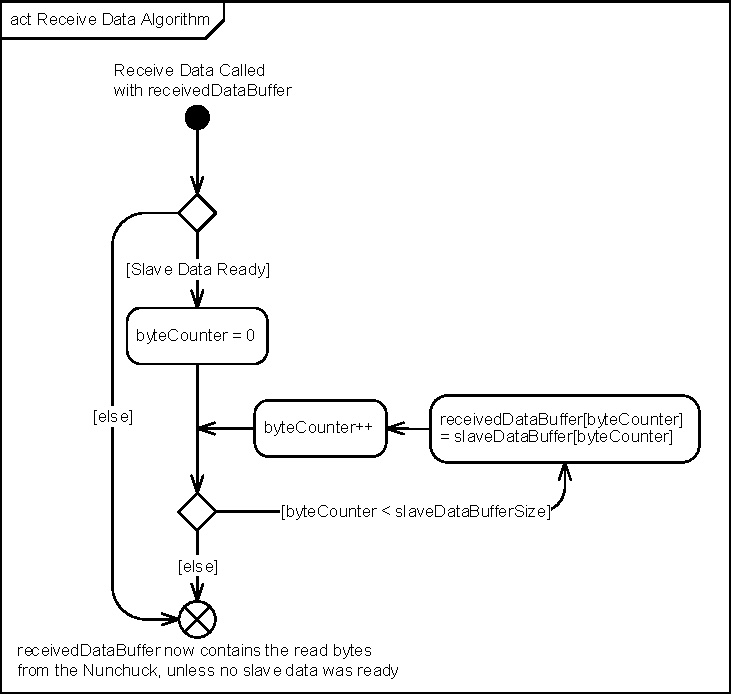
\includegraphics[]{DesignOgImplementering/images/ReceiveDataAlgorithm}
	\caption{Aktivitetsdiagram over \textit{receiveData} metodens algoritme}
	\label{figure:ReceiveDataAlgorithm}
\end{figure}

\noindent Algoritmen starter når funktionen \textit{receiveData} bliver eksekveret. Klienten der kalder funktionen angiver desuden en buffer ved navn \textit{receivedDataBuffer}. Denne buffer udfyldes med den modtagne I2C data. Det bliver tjekket om der er data klar til aflæsning på PSOC'ens I2C modtager buffer. Denne buffer er navngivet \textit{slaveDataBuffer} i aktivitetsdiagrammet. Hvis dette er tilfældet, bliver alle bytes fra \textit{slaveDataBuffer} overført til \textit{receivedDataBuffer}. På denne måde vil \textit{receivedDataBuffer} til slut indeholde alle bytes modtaget fra I2C bussen.

\subsection{Nunchuck}
\label{afsnit:nunchuckDI}
I dette afsnit vil softwaren der specifikt omhandler kommunikationen mellem PSoC0 og Nunchucken blive beskrevet. Dette gøres vha. et klassediagram og klassebeskrivelser.

\subsubsection{Klassediagram}
På figur \ref{figure:NunchuckKlassediagram} ses klassediagrammet for Nunchuck klassen.

\begin{figure}[H]
	\centering
	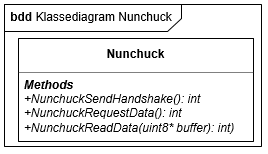
\includegraphics[]{DesignOgImplementering/images/nunchuck}
	\caption{Klassediagram for Nunchuck klassen}
	\label{figure:NunchuckKlassediagram}
\end{figure}

\subsubsection{Klassebeskrivelser}
Metoderne fra klassediagrammet figur \ref{figure:NunchuckKlassediagram} vil blive beskrevet i dette afsnit. \newline

\noindent Nunchuck klassen har til ansvar at læse data fra Wii-Nunchuck controlleren. For at aflæse og dekode data, er formler og andet information taget fra (Bilag/Dokumentation/WiiNunchuck.pdf). \newline

\noindent\textbf{int NunchuckSendHandshake()}\newline
Denne metode sender et \textit{handshake} til Nunchuck enheden. Handshaket bruges til at parre PSoC'en med nunchucken. Metoden returnerer et '0' hvis der opstår en fejl. \newline

\noindent\textbf{int NunchuckRequestData()}\newline
Denne metode sender et 0x00 til nunchuck'en, og derved beder nunchuck'en om at klargøre data til overførsel. Metoden returnerer et '0' hvis der opstår en fejl. \newline

\noindent\textbf{int NunchuckreadData(uint8* buffer)}\newline
Denne metode bruger PSoC Creator's I2C-API til at læse data fra nunchuck'en (data der blev klargjort fra NunchuckRequestData()). Disse data bliver derefter dekrypteret og gemt i "buffer", så de bliver tilgængelige uden for metodens scope. \newline

\noindent I klassediagrammet er der en sektion kaldet \textit{Defines}. Disse Defines bruges i implementeringen til forskellige formål. \textit{PSoC0UnitAddress, PSoC1UnitAddres} og \textit{nunchuckUnitAddress} bruges til at definere adresserne for I2C-nettets slaver. \textit{NunchuckData, I2CTestRequest} og \textit{I2CTestACK} er kommando typer der bruges til at bestemme hvilken kommando type der er blevet sendt/modtaget, og hvor mange bytes der skal forventes at være gemt i databufferen. Se dokumentationen afsnit \ref{afsnit:I2CProtokol} tabel \ref{table:I2CKommandoer}.

\subsubsection{Nunchuck Read Data Algoritme}

På figur \ref{figure:nunchuckReadDataAlgorithm} ses et aktivitetsdiagram for algoritmen der aflæser Nunchuck'ens tilstand ved at modtage dets bytes, for herefter at dekode og kalibrere dem, så værdierne kan bruges til styring og affyring af kanonen.

\begin{figure}[H]
	\centering
	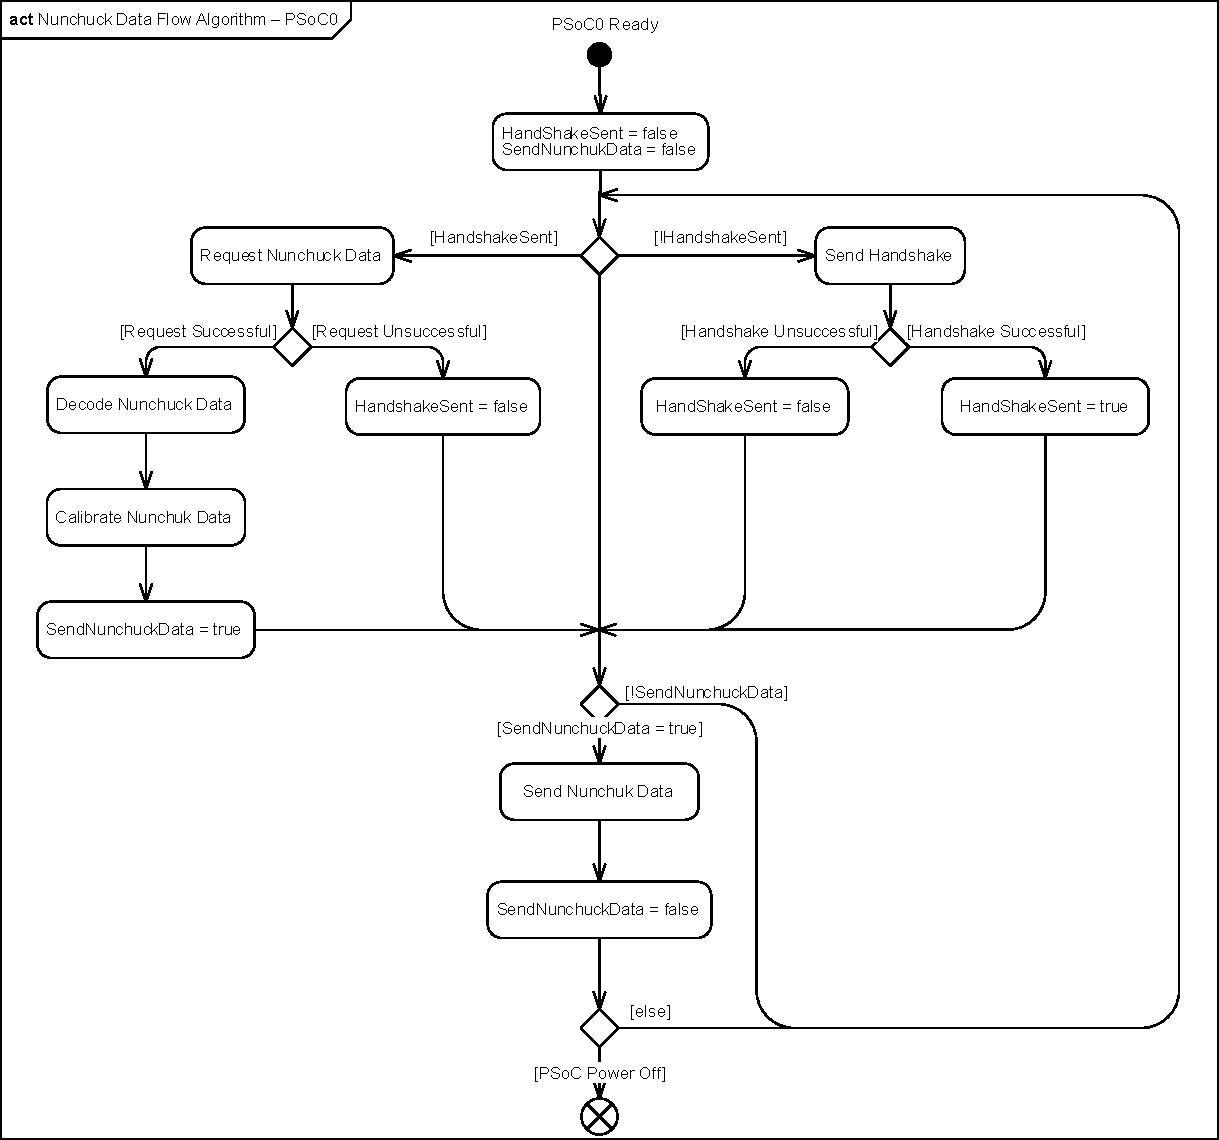
\includegraphics[width=\textwidth]{DesignOgImplementering/images/nunchuckFlowActivity}
	\caption{Aktivitetsdiagram over \textit{NunchuckReadData} metodens algoritme}
	\label{figure:nunchuckReadDataAlgorithm}
\end{figure}

På tabel \ref{table:nunchuckActivityVariables} ses variablerne der indgår i aktivitetsdiagrammet på figur \ref{figure:nunchuckReadDataAlgorithm}.

\begin{table}[H]
	\centering
	\begin{tabular}{|l|l|}
		\hline
		Variable         & Beskrivelse                                                                                                                                              \\ \hline
		HandShakeSent    & \begin{tabular}[c]{@{}l@{}}Denne variabel indikerer om\\ der er sendt et handshake til Nunchuck'en\\ eller ej.\end{tabular}                              \\ \hline
		SendNunchuckData & \begin{tabular}[c]{@{}l@{}}Denne variabel indikerer om der er aflæst\\ data fra Nunchuck som kan videresendes\\ til PSoC1 for motorstyring.\end{tabular} \\ \hline
	\end{tabular}
	\caption{Variable der indgår i aktivitetsdiagrammet figur \ref{figure:nunchuckReadDataAlgorithm}}
	\label{table:nunchuckActivityVariables}
\end{table}

Algoritmen gentager sig selv indtil PSoC'en slukkes, så input fra Nunchuck'en konstant aflæses. Den grundlæggende idé er, at der først tjekkes på om et \textit{handshake} er sendt til Nunchuck'en eller ej, hvilket er et krav for at kunne aflæse data fra den. I tilfældet hvor det ikke er afsendt, vil algoritmen blive ved med at forsøge indtil dette lykkedes. Herefter vil algoritmen kontinuert aflæse data fra Nunchuk'en, dekode det og til sidst kalibrere det. Hvis der er en ukendt årsag ikke kan aflæses data, bliver \textit{handshakeSent} sat til false. \newline

\noindent Hvis der til slut er Nunchuck data at sende, vil denne data blive afsendt til PSoC1, og \textit{SendNunchuckData} sættes til false, så en aflæsning sker igen.

\subsection{Rotationsbegrænsning}
I forbindelse med begrænsning af motorens rotation er der nogle indstillinger der skal sættes, se afsnit \ref{afsnit:rotationsbegraensning}. ADC'en skal indstilles til at gøre brug af en kanal i single mode, da der ét inputsignal fra potentiometret og denne skal bestemmes i forhold til stel. For at styre motorens bevægelse i et interval er følgende algoritme implementeret.

\begin{figure}[H]
	\centering
	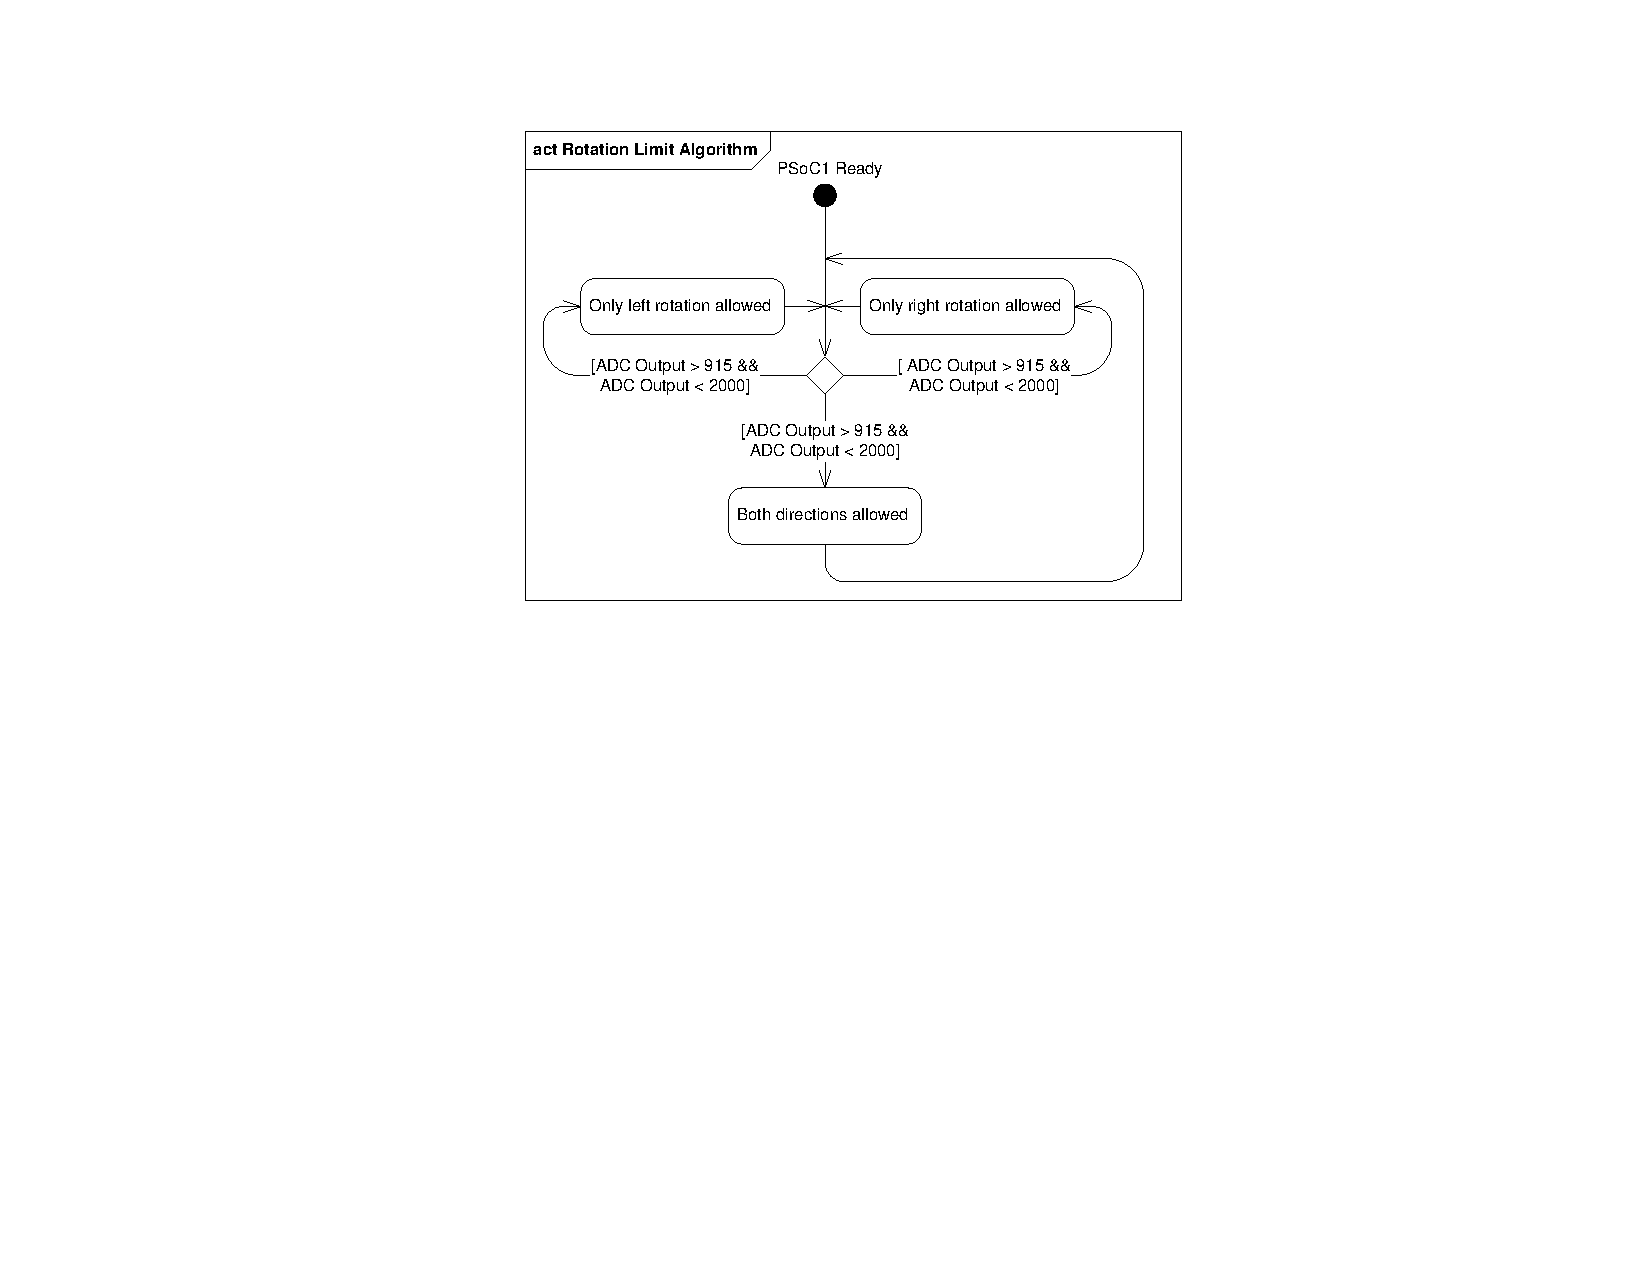
\includegraphics[width=\textwidth]{DesignOgImplementering/images/rotationalgorithm}
	\caption{Aktivitetsdiagram for rotationsbegrænsningsalgortimen}
	\label{fig:rotation}
	
\end{figure}

\noindent På figur \ref{fig:rotation} ses et aktivitetsdiagram for algoritmen for rotationsbegrænsning. Der er fastsat to værdier for ydergrænser. Når motoren bevæger sig udover ydergrænserne, blokeres motoren for den givne retning indtil motoren er tilbage i intervallet. 

\subsection{Motorstyring}
Til styring af motorene gøres der brug af fire PWM blokke, to til styring af X-aksen og to til styring af Y-aksen, se afsnit \ref{afsnit:H-bro}. Disse PWM blokke er indstillet med en clock frekvens på 3MHz. Til styring af motorene er følgende algoritme implementeret. 
\begin{figure}[H]
	\centering
	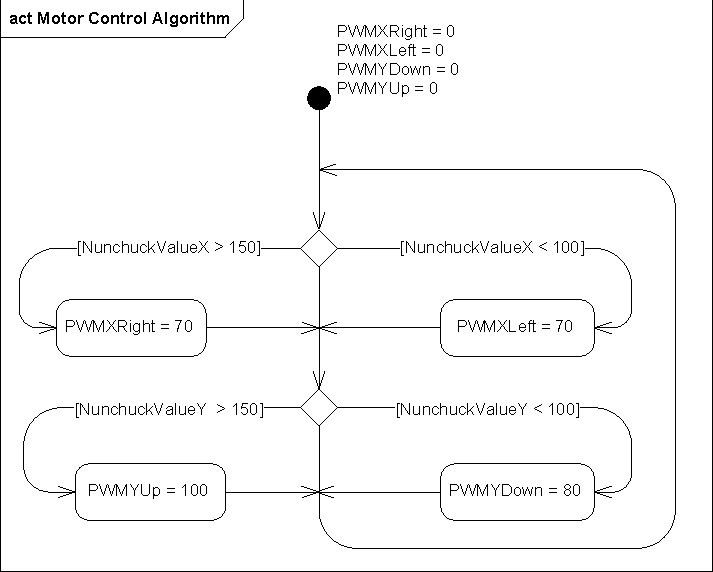
\includegraphics[scale=0.8]{DesignOgImplementering/images/motorcontrolalgorithm}
	\caption{Aktivitetsdiagram for motorstyringsalgortimen}
	\label{fig:motorstyringal}
\end{figure}

\noindent På figur \ref{fig:motorstyringal} ses aktivitetsdiagrammet for motorstyringsalgoritmen. Der ses at retningensignalerne bestemmes ud fra Wii-Nunchuck'ens inputværdier fra X- og Y-aksen.

% % % % % % % % % % % % PSoC2 % % % % % % % % % % % % % % % % % % % % % % % %
\subsection{Affyringsmekanisme}
\label{afsnit:affyringsmekanisme}
PSoC2 anvendes til styring af affyringsmekanismen. Til rotationsdetektorens operationsforstærker er der anvendt en, der er indbygget i PSoC'en. Derudover styres bl.a. interrupt og PWM-signaler i forbindelse med affyringsmekanismen ved hjælp af PSoC2. Desuden aflæses spændingen fra rotationsdetektoren af en SAR ADC, som også findes på PSoC2. Til at håndtere affyringen er der opstillet en kodesekvens, som køres ved modtagelse af et interrupt. Et sekvensdiagram for afviklingen af koden i interruptet ses på figur \ref{fig:aktivitetsdiagramDetektor}. \\

\begin{figure}[H]
	\centering
	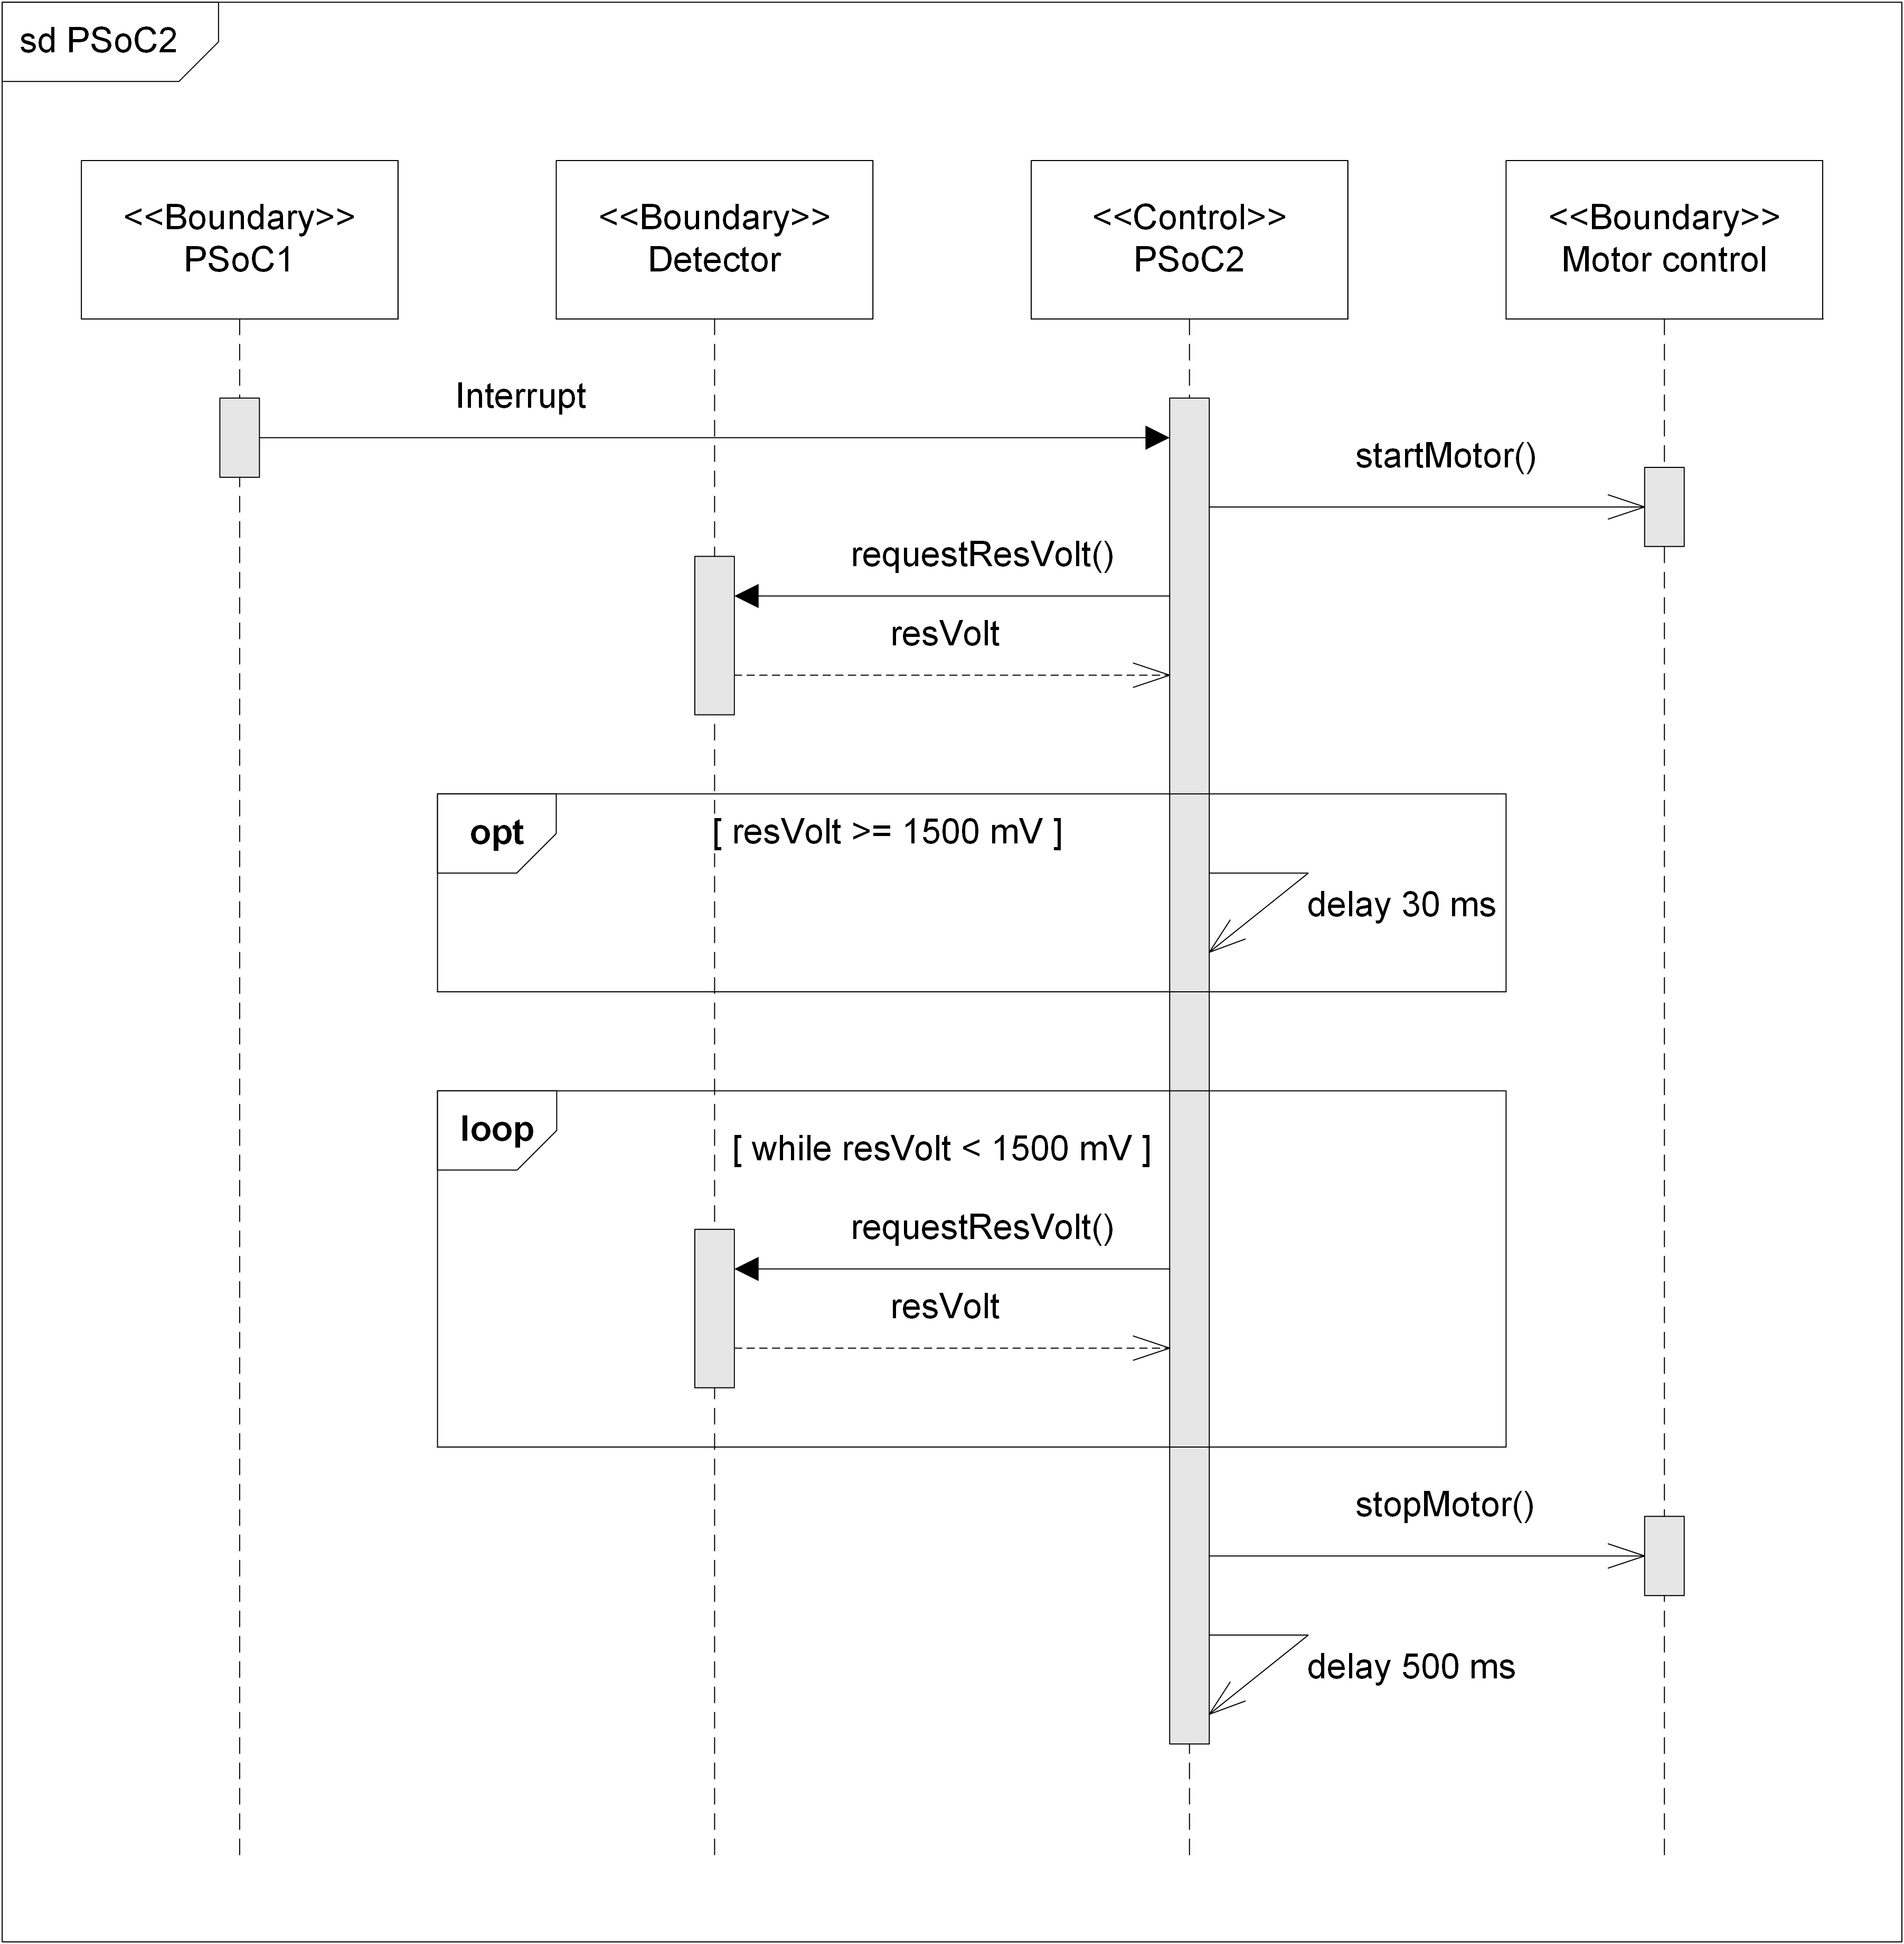
\includegraphics[width=1\textwidth]{Afsnit/DesignOgImplementering/images/PSoC2sekvens.png}
	\caption{Sekvensdiagram for PSoC2 software ved affyring af kanonen} 
	\label{fig:aktivitetsdiagramDetektor}
\end{figure}

\noindent For at affyringssekvensen initieres, skal der modtages et interrupt. Det sker, når brugeren affyrer kanonen, og PSoC1 sender et højt signal, som går ind på en inputpind på PSoC2, som så er programmeret til at trigge på rising edge og derved køre interruptrutinen. \newline

\noindent Det første der sker i interruptrutinen er, at ADC-værdien aflæses som en spænding i millivolt. Blokken til ADC'en, som er anvendt i koden ses på figur \ref{fig:PSoC2blokke}, og hvilke porte på PSoC2, de er forbundet til ses på figur \ref{fig:PSoC2ports}. Spændingen fra ADC'en lægges over i variablen "resVolt". Så startes motoren, derved begynder kanonen at affyre. PSoC'ens røde LED er af debugginghensyn som udgangspunkt tændt, når der ikke affyres, når interruptet kommer, slukkes den, og den grønne PSoC-LED tændes i stedet, for til debugging at indikere, at interruptrutinen køres.


\begin{figure}[H]
	\centering
	\includegraphics[width=2.7\textwidth, trim={5cm 5.7cm 0 4.3cm}]{Afsnit/DesignOgImplementering/images/PSoC2blokke}
	\caption{PSoC2 software PSoC-blokke} 
	\label{fig:PSoC2blokke}
\end{figure}


\noindent Dernæst anvendes spændingen fra resVolt, der blev aflæst fra ADC'en så til at vurdere om fotodioden, kan se lyset fra den røde LED. Når de ikke kan se hinanden er spændingen 500 mV, og når de kan se hinanden er spædningen mellem 4000 og 5000 mV. Normalt indikerer det, at de kan se hinanden, at affyringen er færdig, og at motoren skal stoppes, men hvis de kan se hinanden på dette tidspunkt ved interruptets start, betyder det, at de, inden affyringen er startet, allerede er placeret så de kan se hinanden. Hvis det er tilfældet køres et delay på 30 ms, for at sikre at motoren er drejet, så de igen ikke kan se hinanden. Derefter aflæses spændingen ved ADC'en igen - nu for at tjekke om affyringen er afsluttet. 

\begin{figure}[H]
	\centering
	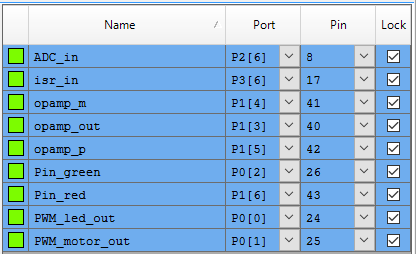
\includegraphics[width=0.7\textwidth]{Afsnit/DesignOgImplementering/images/PSoC2porte}
	\caption{PSoC2 ports for software pins} 
	\label{fig:PSoC2ports}
\end{figure}

\noindent Aflæsningen gentages indtil fotodioden kan se den røde LED, og motoren dermed skal stoppes. Affyringen sker på langt under et sekund, og det er derfor ikke problematisk med polling. Alternativt, hvis affyringen varede længere tid, kunne det have været implementeret med et interrupt, men i dette tilfælde kan det klares ved at tjekke ADC'en flere gange. \newline

\noindent Når motoren er stoppet, slukkes den grønne debugging PSoC-LED, og der køres et delay på 500 ms, så der går et halvt sekund, inden der igen kan skydes. Derved undgås det, at kanonen affyres med det samme igen, hvis triggeren ved en fejl ikke er sluppet. Som det sidste tændes den røde PSoC LED, som ved debugging indikerer, at kanonen igen er klar til at blive affyret. \newline

\noindent Både PWM-signalet til affyring af motoren og til generering af 10 kHz til den røde LED styres af PSoC2. De to PWM-blokke deles om en clock, der er sat til en frekvens på 2,5 MHz. Forbindelsen mellem clock'en og PWM-blokkene ses på figur \ref{fig:PSoC2blokke}, og hvilke porte PWM-blokkenes udgange er forbundet til ses på figur \ref{fig:PSoC2ports}. PWM til den røde LED, har en periode på 250, dermed bliver PWM-signalet 10 kHz, som det også ses af ligning \ref{eq:yndlingsligning}.

\begin{align}
f_{LED} = \frac{f_{clock}}{periode_{LED}} \label{eq:yndlingsligning}
\end{align}

\begin{align}
f_{LED} = \frac{2,5 MHz}{250}\nonumber
\end{align}

\begin{align}
f_{LED} = 10 kHz \nonumber
\end{align}

\noindent Derudover er dutycyclen for LED'en 10 \%. PWM-signalet til motoren har en periode på 75, derved bliver frekvensen 33,33 kHz. Beregningen for dette ses på ligning \ref{eq:fmotor}. En DC-motor skal gerne styres af et PWM-signal på over 20 kHz, for at rotere uden problemer. Dermed passer de 33,33 kHz godt. 

\begin{align}
f_{LED} = \frac{f_{clock}}{periode_{motor}} \label{eq:fmotor}
\end{align}

\begin{align}
f_{LED} = \frac{2,5 MHz}{75}\nonumber
\end{align}

\begin{align}
f_{LED} = 33,33 kHz \nonumber
\end{align}

\section{Afkodning af Wii-Nunchuck Data Bytes}
Aflæste bytes fra Wii-Nunchuck - indeholdende tilstanden af knapperne og det analoge stick - er kodet når de oprindeligt modtages via I2C bussen. Disse bytes skal altså afkodes før deres værdier er brugbare. Afkodningen af hver byte sker ved brug af følgende formel (Bilag/Dokumentation/WiiNunchuck.pdf): \newline
\noindent \textit{AfkodetByte = (AflæstByte XOR 0x17) + 0x17} \newline

\noindent Fra formlen kan det ses at den aflæste byte skal \textit{XOR}'s med værdien 0x17, hvorefter dette resultat skal adderes med værdien 0x17.

\section{Kalibrering af Wii-Nunchuck Analog Stick}
De afkodede bytes for Wii-Nunchuck's analoge stick har definerede standardværdier for dets forskellige fysiske positioner. (Bilag/Dokumentation/WiiNunchuck.pdf) Disse værdier findes i tabel \ref{tabel:WiiNunchuckStickPositioner}

\begin{table}[H]
	\centering
	\begin{tabular}{|l|l|}
		\hline
		X-akse helt til venstre & 0x1E \\ \hline
		X-akse helt til højre   & 0xE1 \\ \hline
		X-akse centreret        & 0x7E \\ \hline
		Y-akse centreret        & 0x7B \\ \hline
		Y-akse helt frem        & 0x1D \\ \hline
		Y-akse helt tilbage     & 0xDF \\ \hline
	\end{tabular}
	\caption{Standardværdier for fysiske positioner af Wii-Nunchuck's analoge stick}
	\label{tabel:WiiNunchuckStickPositioner}
\end{table}

\noindent I praksis skal de afkodede værdier for det analoge stick kalibreres, da slør pga. brug gør at de ideale værdier ikke rammes. \newline

\noindent I projektet er de afkodede værdier for det analoge stick kalibreret med værdien -15 (0x0F i hexadecimal), altså ser den endelige formel for afkodning samt kalibrering således ud: \newline

\noindent \textit{AfkodetByte = (AflæstByte XOR 0x17) + 0x17 - 0x0F}

\section{Hardwaredesign}
På baggrund af BDD'et er der fundet følgende hardwareblokke, der skal udarbejdes: 

\begin{itemize}
	\item Tre motorer
	\item Motorstyring
	\item Affyringsmekanisme 
\end{itemize}

Disse beskrives i de følgende afsnit. 

\subsection{Motor}
Der er valgt at bruge en DC-motor i alle tre tilfælde \cite{legoMotor}. De to motorer skal bruges til at styre kanonen i to akser, og den sidste skal bruges i affyringsmekanismen. 

\subsection{Motorstyring}
Motorstyringen skal sørge for at kanonen kan styres i de vertikale og horizontale
akser samt begrænse platformens rotation. Til at bevæge kanonen bruges to
DC motorer, en til hver akse. Disse motorers rotationsretning styres med en
H-bro. For at sikre at platformen ikke kan roteres 360 grader, er der udviklet
en rotationsbegrænsning.

\subsubsection{H-bro}
\label{afsnit:H-bro}
Der blev først designet en H-bro, som bestod af to N-MOSFET's af typen IRLZ44(Bilag/Dokumentation/IRLZ44.pdf) og to P-MOSFET's af typen ZVP3306A. Det viste sig dog, at den P-MOSFET, der var brugt, ikke kunne klare strøm, som motoren skulle bruge, hvilket betød, at den blev brændt af. Derfor blev denne H-bro modificeret, så de to P-MOSFET's blev udskiftet med to MOSFET's af typen IRF9Z34N(Bilag/Dokumentation/irf9z34n p mosfet.pdf), der kan trække en større strøm. 

\begin{figure}[H]
	\centering
	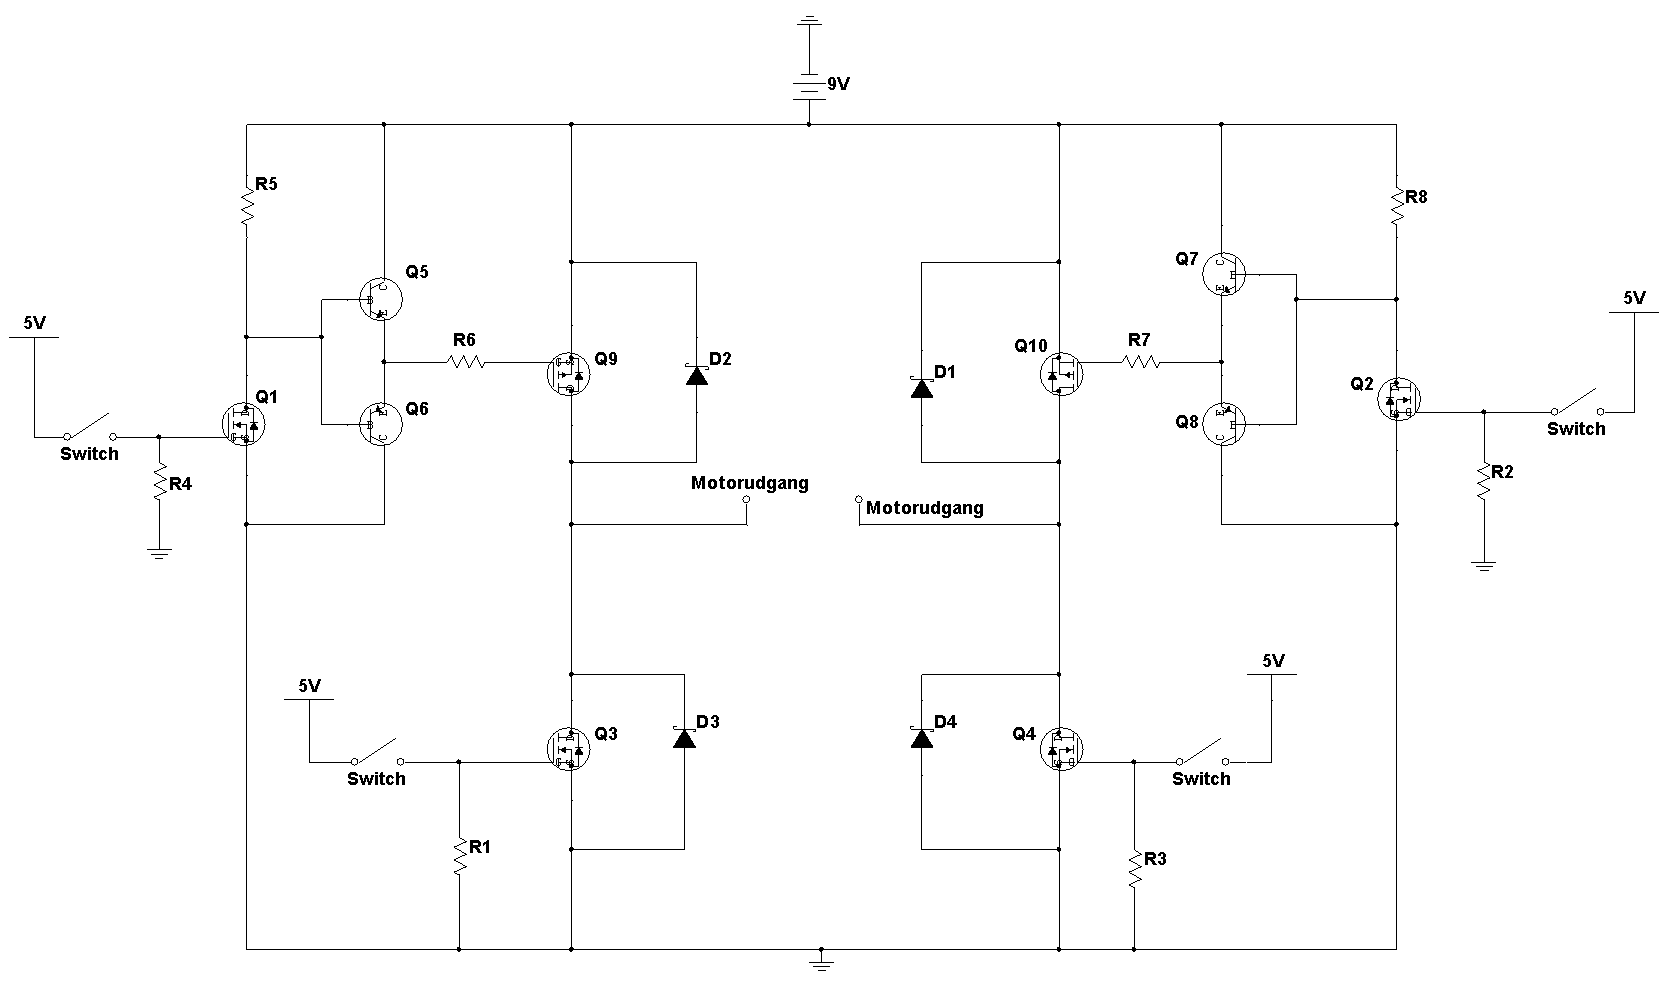
\includegraphics[width=\textwidth]{DesignOgImplementering/images/H-bro}
	\caption{Multisim kredsløb for H-bro}
	\label{fig:hbro}
	\end{figure}

\begin{table}[H]
	\centering
	\begin{tabular}{|l|l|l}
		\cline{1-2}
		Betegnelse 	& Komponent 	          	 &  \\ \cline{1-2}
		Q1   		& IRLZ44 (MOSFET N-kanal)   &  \\ \cline{1-2}
		Q2   		& IRLZ44 (MOSFET N-kanal)   &  \\ \cline{1-2}
		Q3   		& IRLZ44 (MOSFET N-kanal)   &  \\ \cline{1-2}
		Q4   		& IRLZ44 (MOSFET N-kanal)   &  \\ \cline{1-2}
		Q5   		& BC547                      &  \\ \cline{1-2}
		Q6   		& BC557                      &  \\ \cline{1-2}
		Q7   		& BC547                      &  \\ \cline{1-2}
		Q8   		& BC557                      &  \\ \cline{1-2}
		Q9   		& IRF9Z34N (MOSFET P-kanal) &  \\ \cline{1-2}
		Q10  		& IRF9Z34N (MOSFET P-kanal) &  \\ \cline{1-2}
		R1   		& 10k$\Omega$                &  \\ \cline{1-2}
		R2   		& 10k$\Omega$                &  \\ \cline{1-2}
		R3   		& 10k$\Omega$                &  \\ \cline{1-2}
		R4   		& 10k$\Omega$                &  \\ \cline{1-2}
		R5   		& 10k$\Omega$                &  \\ \cline{1-2}
		R6   		& 100$\Omega$                &  \\ \cline{1-2}
		R7   		& 100$\Omega$                &  \\ \cline{1-2}
		R8   		& 10k$\Omega$                &  \\ \cline{1-2}
		D1   		& IN5819						&  \\ \cline{1-2}
		D2   		& IN5819						&  \\ \cline{1-2}
		D3   		& IN5819						&  \\ \cline{1-2}
		D4   		& IN5819		              &  \\ \cline{1-2}
	\end{tabular}
	\caption{Komponentbetegnelser på H-bro}
	\label{hbrotabel}
\end{table}

\begin{itemize}
\item MOSFET'er \\
Til at styre motoren er der bygget en H-bro, som består af fire mosfet, hvor to af dem er af typen IRF9Z34N (mosfet P-channel, som er Q9 og Q10 på figur \ref{fig:hbro}) og de to andre mosfet er af typen IRLZ44 (mosfet N-Channel, som er Q3 og Q4 på figur \ref{fig:hbro}). Det er valgt at bruge mosfet for at kunne styre H-broen, da det ved denne er muligt at lukke og åbne for spændingen, og de bliver styret af spænding, i forhold til transistorer, som bliver styret af strøm. 

\begin{itemize}
\item MOSFET N-kanal \\
	Der er i denne H-bro brugt en N-kanals-MOSFET af typen IRLZ44 (Bilag/Dokumentation/IRLZ44.pdf). Denne MOSFET skal bruges til at trække spændingen fra den tilsvarende P-MOSFET til stel, så motoren kan begynde at køre. Det sker, når der kommer 5V ind på gate-benet. 
	\\MOSFET'en fungerer på den måde, at når der kommer positiv spænding ind på gate-benet åbner den, så der kommer forbindelse til stel og når der kommmer 0V ind på dette lukker den igen. 
	
	\begin{figure}[H]
		\centering
		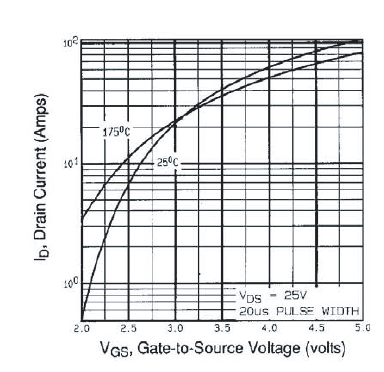
\includegraphics[width=\textwidth]{DesignOgImplementering/images/grafn}
		\caption{Gate-to-Source Voltage(Bilag/Dokumentation/IRLZ44.pdf)}
		\label{fig:mosfetn}
	\end{figure}
	
	På figur \ref{fig:mosfetn} ses det, at når der er en gate-to-source-spænding på 5V, vil der MOSFET'en kunne klare, at der løber en strøm på op til 100A i følge datablad(Bilag/Dokumentation/IRLZ44.pdf). Det vil altså ikke komme til at påvirke motoren, da denne kun kan trække en strøm på cirka 60mA. 
	
\item MOSFET P-kanal \\
	Der er valgt at bruge en P-MOSFET af typen IRF9Z34N (Bilag/Dokumentation/irf9z34n p mosfet.pdf). Denne MOSFET skal bruges til at trække de 9V ned til motoren, så denne kan køre. Samtidig sørger den for, at de 9V ikke løber ned til motoren så længe, der ikke er negativ spænding på gate-benet. 
	Denne type MOSFET kan trække en strøm på 6,7A ifølge databladet (Bilag/Dokumentation/irf9z34n p mosfet.pdf). Det vil altså ikke komme til at påvirke motoren, da den kun kan trække en strøm på cirka 60mA. 
	
	For at der kan løbe spænding igennem IRF9Z34N, skal den have en negativ spænding for at åbne og en spænding på over 0V for at lukke. 
	
	\begin{figure}[H]
		\centering
		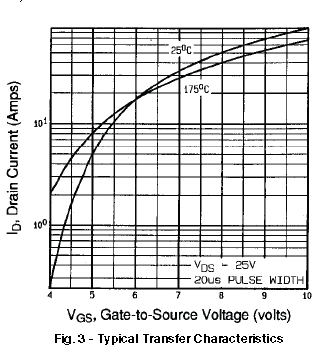
\includegraphics[width=\textwidth]{DesignOgImplementering/images/grafp}
		\caption{Gate-to-Source Voltage (Bilag/Dokumentation/irf9z34n p mosfet.pdf)}
		\label{fig:mosfetp}
	\end{figure}
	
	\noindent På figuren \ref{fig:mosfetp} ses det, at når der er en gate-to-source-spænding på 5V, vil der kunne løbe en strøm på omkring 5A igennem MOSFET'en, hvilket er mere end nok til at få motoren til at køre. 
\end{itemize}

\item Dioder \\
Som det se på figur \ref{fig:hbro} er der sat en diode af typen IN5819 (Bilag/Dokumentation/1N5819.pdf) over fire af MOSFET'ene (Q9, Q10, Q3 og Q4). Disse skal fungere som beskyttelse af MOSFET'en. Det, dioden gør, er, at den sikrer, at den spænding, som er tilbage i motoren, når der lukkes for MOSFET'en, ikke løber tilbage ind i MOSFET'en og brænder den af.

\item Modstande
\begin{itemize}
	\item Pull down modstande:\\
	Der er blevet brugt fire pull-down-modstande (R1, R2, R3 og R4 som ses på figur \ref{fig:hbro}). Disse sørger for, at signalet vl blive holdt lavt, når der ikke sendes signal ind på MOSFET'ens gateben. Hvis der blev sendt signal ind imens der også blev sendt signal ind fra den anden side af H-broen ville MOSFET'en blive brændt af. Altså skal modstanden være lille nok til, at de små spændinger kan løbe til stel, når der ikke er PWM-signal, men samtidig stor nok til, at spændingen ikke løber til stel, når der er signal på gatebenet. Der er derfor valgt en modstand med en værdi på $10k\Omega$. 
	
	\item Andre modstande
	\begin{itemize}
		\item R6 og R7\\
			Grunden til, at R6 og R7(på figur \ref{fig:hbro}), er der, er for at sikre, at transistorernes Absolute Maximum Ratings omkring strømmen, som ikke må overstige 100mA ifølge databladet (Bilag/Dokumentation/BC557.pdf) og (Bilag/Dokumentation/BC547.pdf)
		
		\begin{displaymath}
			R6=R7=\frac {9V}{100mA} =90\Omega
		\end{displaymath}
		Der blev valgt en modstand med en værdi på 100$\Omega$ i stedet, for at være på den sikre side. 
		
		\item R5 og R8 (jf. figur \ref{fig:hbro})\\
		Grunden til at R5 og R8 er indsat i kredsløbet er, at der ifølge databladet kun kan løbe en strøm på omkring 30A igennem N-MOSFET, hvis Vgs er på 10V. Da Vgs, i  dette projekt, kun er sat til 5V, vil MOSFET'en altså ikke kunne klare en alt for stor strøm. Derfor er R5 og R8 sat ind for at forhindre, at MOSFET'en ikke brænder af. (Bilag/Dokumentation/IRLZ44.pdf).
		
		Der blev fundet en modstand ved at regn med at der 9V og at mosfet kun kan klar en strøm under 30A så der blev regnet med de 30 A selv om man vidste godt det ikke var det som den kunne klare, men der skulle en større modstand ind, men det var så man havde noget at gå ud fra 
		\begin{displaymath}
		R8=R5=\frac {9V}{30A} =0.3\Omega
		\end{displaymath}
		
		
		0.3 var alt for lille så der blev prøvet op end til der blev fundet en som passet, hvor det blev en på 10K så er man sikker på der ikke sker noget med mosfet’en 
		
		
	\end{itemize}
\end{itemize}

\item Transistorer
\begin{itemize}
	\item Q5 og Q7(Bilag/Dokumentation/BC557.pdf) (jf. figur \ref{fig:hbro})
	Disse transistorer sidder i kredsløbet, fordi det tager tid for P-MOSFET'en at blive opladt helt og dermed åbne helt, på grund af kondensatoreffekten mellem benene på MOSFET'en.
	
	\item Q6 og Q8(Bilag/Dokumentation/BC547.pdf) (jf. figur \ref{fig:hbro})
	Disse to transistorer sidder der for at hjælpe med at lukke P-MOSFET'en igen. Inden Q5 og Q7 blev sat ind tog det tid for at lukke P-MOSFET'en, men da de to blev sat ind, kunne de hjælpe til med at aflade MOSFET'en hurtigere. 
\end{itemize}
\end{itemize}

\subsubsection{Rotationsbegrænsning}
\label{afsnit:rotationsbegraensning}
Platformen, som styres af motoren, må ikke kunne rotere 360 grader. Dette ses i ikke funktionelle krav, afsnit \ref{afsnit:ikkeFunkKrav}. For at begrænse motorens bevægelse, anvendes et potentiometer samt en ADC. Når motoren bevæger sig, ændres potentiometerets modstandsværdi, og dermed ændres spændingsniveauet. På figur \ref{fig:opstillingADC} ses den endelige opstilling af rotationsbegrænsningen.

\begin{figure}[H]
	\centering
	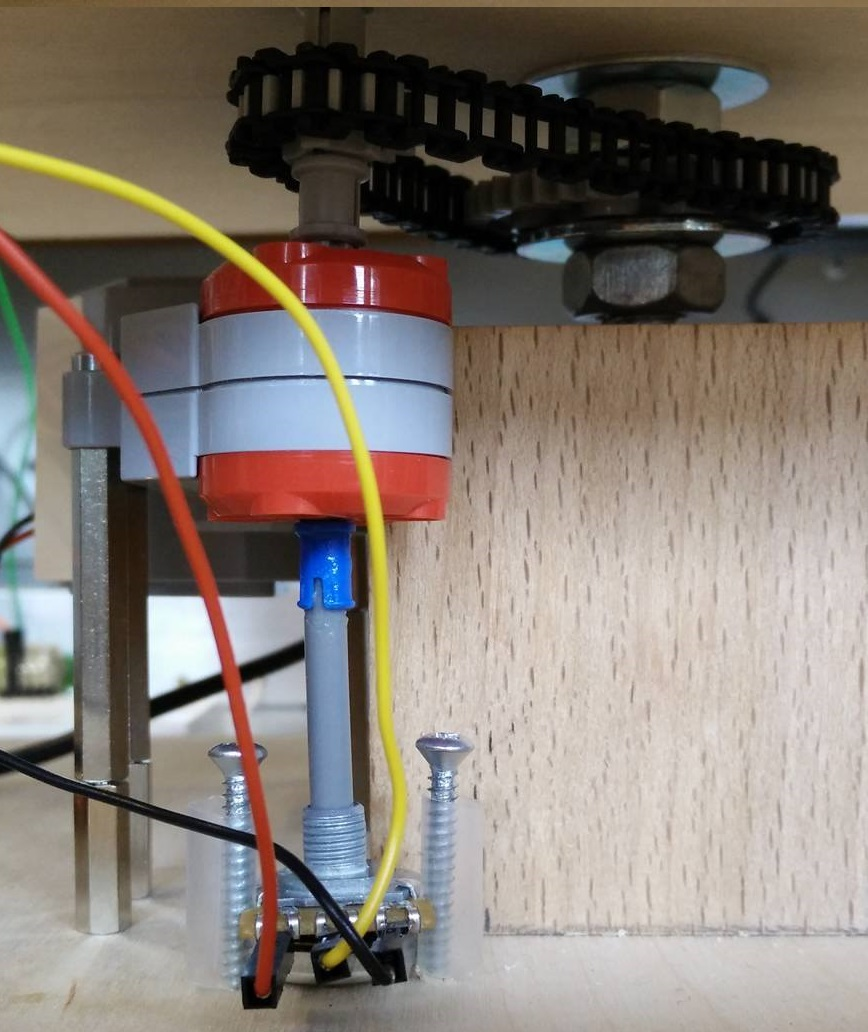
\includegraphics[scale=0.3]{Afsnit/DesignOgImplementering/images/potentiometerADC}
	\caption{Opstilling for rotationsbegrænsning}
	\label{fig:opstillingADC}
\end{figure}

\noindent \textbf{Potentiometer} \newline
\noindent Den første del af rotationsbegrænsningen er et potentiometer, som fungerer efter spændingsdelerprincippet, som vist på figur \ref{fig:potentiometer2}.

\begin{figure}[H]
	\centering
	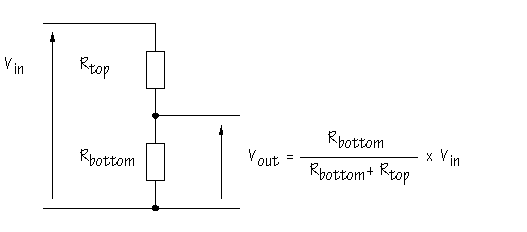
\includegraphics[scale=0.65]{DesignOgImplementering/images/potentiometer}
	\caption{Spændingsdeler formlen for potentiometeret}
	\label{fig:potentiometer2}
\end{figure}

\noindent Det anvendte potentiometer har en størrelse på 47\(\ K\Omega\). Denne er lineær. Det vil sige at spændingen stiger proportionalt med modstanden. I potentiometeret findes en roterende kontakt, der danner en justerbar spændingsdeler. Når skaftet på potentiometret roteres ændres modstanden i de to variable modstande, \(\ R_{1}\) og  \(\ R_{2}\). På figur \ref{fig:potentiometer2} ses en konceptuel afbildning af de variable modstande i potentiometret, hvor der ses at udgangsspændingen er spændingen over \(\ R_{1}\). \newline

\noindent \textbf{ADC} \newline
For at kunne aflæse spændingen på potentiometeret, anvendes en 12-bit AD converter(Bilag/Dokumentation/ADC\_SAR\_SEQ\_P4\_v2\_30.pdf) af typen Sequencing Successive Approximation ADC. En sequencing SAR ADC indeholder et sample-hold kredsløb. Kredsløbet holder på et indgangssignal indtil det næste signal registres på kredsløbets indgang. Dermed har converteren tid til at bestemme outputværdien. \newline \newline
\noindent ADC'en fungerer ved at midscale indstilles til halvdelen af referencespændingen. Inputsignalet sammenlignes med midscale, hvis inputsignalet er højere end midscaleværdien sættes MSB 1 og hvis signalet er lavere bliver denne sat til 0. Herefter bliver midscale værdien rekursivt sat til havdelen af intervallet, som inputsignalet ligger indenfor, og bittene ned til LSB bliver sat. Bittene der sættes, bliver gemt i et register. Når konverteringen er gennemført, kan værdien af inputsignalet aflæses i dette register. 

\begin{figure}[H]
	\centering
	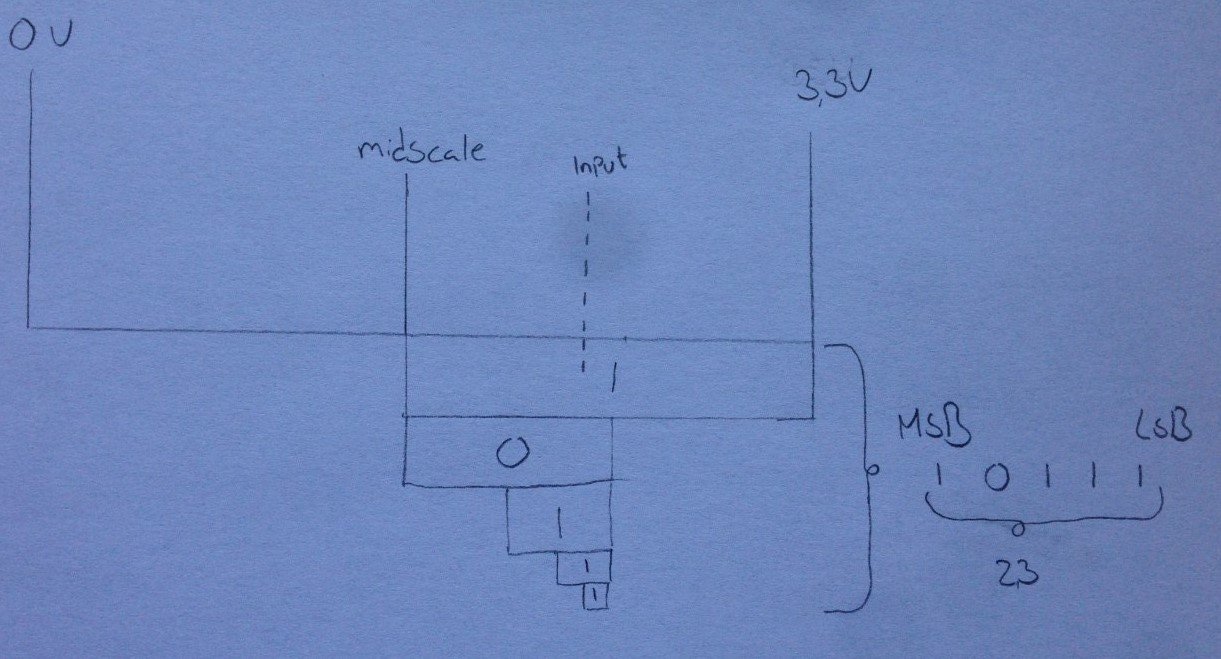
\includegraphics[width=\textwidth]{DesignOgImplementering/images/ADC}
	\caption{Illustation af AD konvertering}
	\label{fig:ADC1}
	
\end{figure}

\noindent På figur \ref{fig:ADC1} ses et eksempel over de første fem trin i en konvertering. Til dette projekt arbejdes der med en 12-bit AD converter, dermed ville denne konvertering forsætte 12 trin ned. 

\subsection{Affyringsmekanisme}
Affyringsmekanismen består af en motor; et motorstyringskredsløb; et detektorkredsløb, der skal detektere, at motoren kun kører en enkelt omgang, når der skydes; og en kanon, som er bygget op af noget mekanik og LEGO. 

\subsubsection{Rotationsdetektor}
Når kanonen affyres, styres det af motoren, og som mekanikken er opbygget, er der et proportionelt forhold mellem omdrejning på motoren og antal skud, der affyres. Derfor er det væsentligt at vide, hvornår motoren har roteret en runde, så den kan stoppes, inden der igen skydes. Til det formål anvendes detektoren. Billedet på figur \ref{fig:detektor} illustrerer hvordan detektoren anvendes.

\begin{figure}[H]
	\centering
	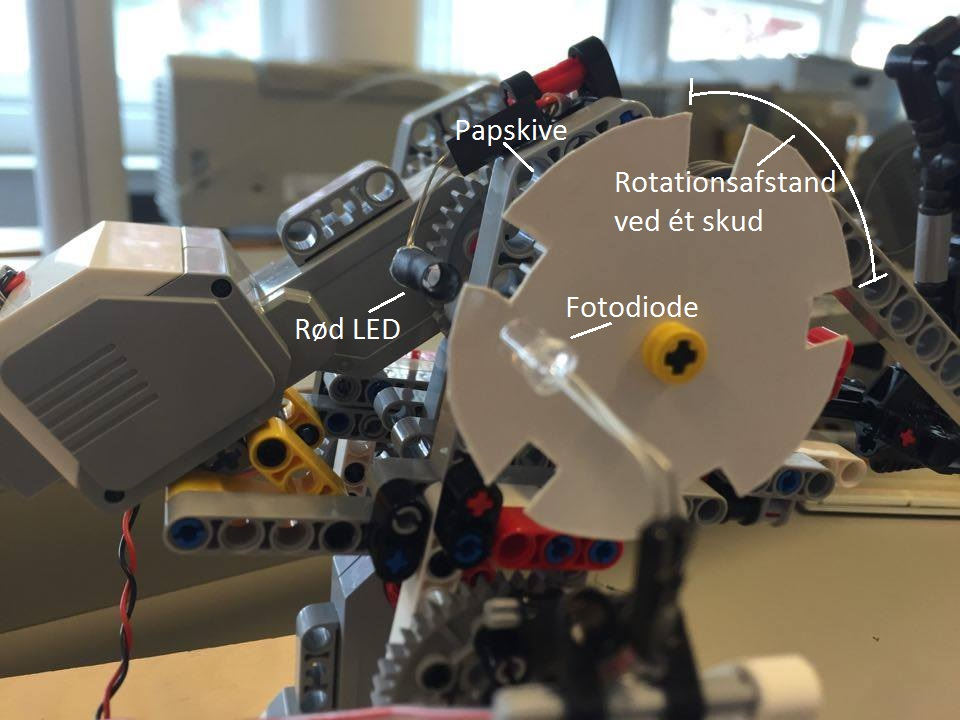
\includegraphics[width=\textwidth]{Afsnit/DesignOgImplementering/images/detektor}
	\caption{Detektorens placering på affyringsmekanismen}
	\label{fig:detektor}
\end{figure}

\noindent Den røde LED og fotodioden anbringes på affyringsmekanismen, som det ses på figur \ref{fig:detektor}. De vender ind mod hinanden, men er adskilt af papskiven. Papskiven er forbundet til motorens rotation, og hver gang et af papskivens hakker roterer forbi dioderne, kan de se hinanden. Fotodioden sender derefter et signal, som kan bruges til at stoppe motoren. Hvert hak passer med, at der er blevet affyret et skud.  \newline

\noindent Detektoren skal kun sende et signal, når fotodioden ser lyset fra LED'en. Det er derfor vigtigt, at den ikke bliver forstyrret af dagslys og andre lyskilder. For at sikre dette, styres den røde LED af et PWM-signal, så LED'en blinker med en frekvens på 10 kHz. Detektoren opbygges tilsvarende af et båndpasfilter, med en centerfrekvens på 10 kHz, som sorterer andre frekvensområder og DC-signaler fra. 10 kHz er rigeligt højt, til at det for øjet ikke er synligt at LED'en blinker. Samtidig er det ikke for højt til, at en almindelig operationsforstærker kan håndtere det. På figur \ref*{fig:detektortand} ses et kredsløbsdiagram for detektoren og LED'en.

\begin{figure}[H]
	\centering
	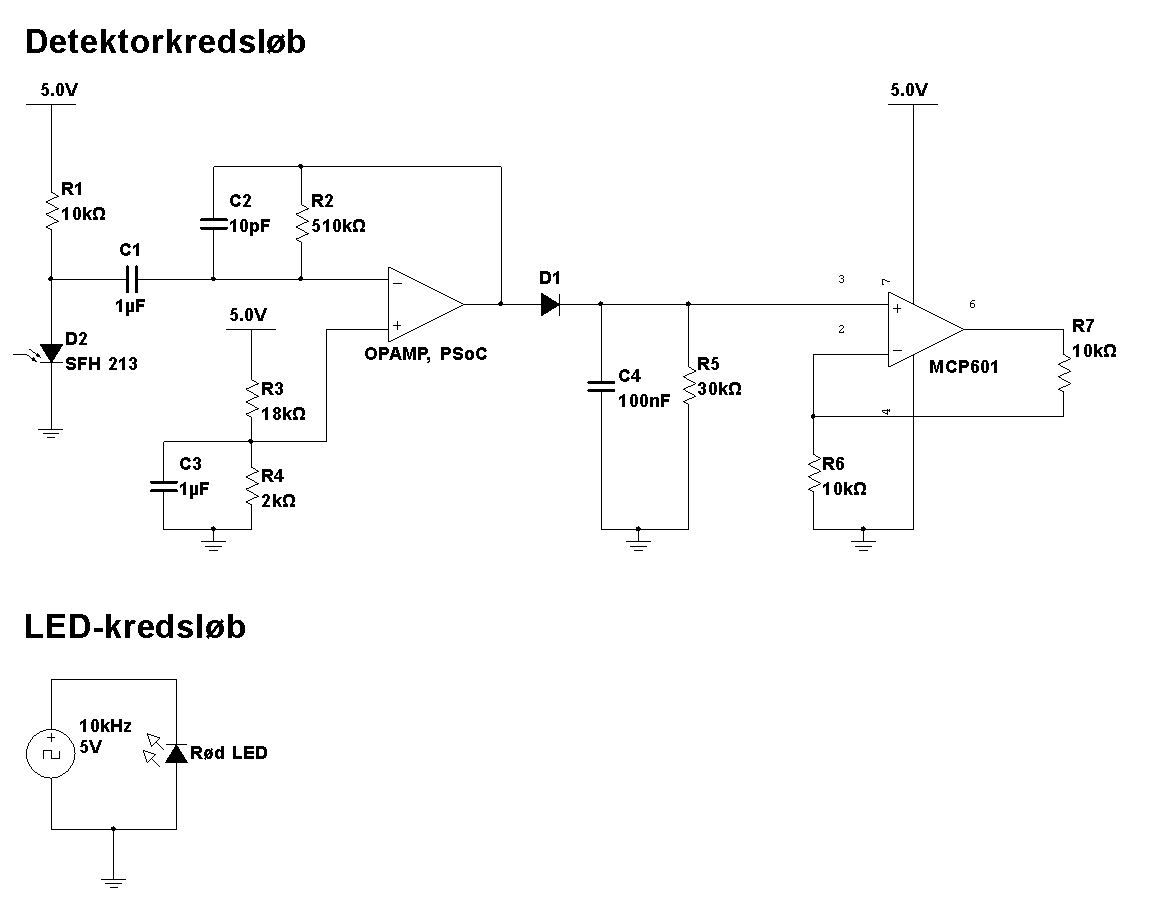
\includegraphics[width=\textwidth]{Afsnit/DesignOgImplementering/images/detektor_tandhjul}
	\caption{Kredsløbsdiagram for detektoren}
	\label{fig:detektortand}
\end{figure}

\noindent Båndpasfiltret er opbygget af et højpasfilter, et lavpasfilter og en operationsforstærker. Da PSoC'en har en indbygget operationsforstærker, anvendes denne. Software design og implementering af den ses under afsnit \ref{afsnit:affyringsmekanisme}. Højpasfilterets afskæringsfrekvens er beregnet på følgende måde: \\

%%%%%Højpasfilter cutoff%%%%
\begin{equation}
	f_{H}=\frac{1}{2\pi R_{H} C_{H}}=\frac{1}{2\pi \cdot 10k\Omega \cdot 1\mu F}=15,9Hz
	\label{cutoffhojpas}
\end{equation} \\

Og lavpasfilterets afskæringsfrekvens er beregnet på følgende måde: \\

%%%%Lavpasfilter cutoff%%%%%
\begin{equation}
	f_{L} = \frac{1}{2\pi R_{L} C_{L}}=\frac{1}{2\pi \cdot 510k\Omega \cdot 10pF}=31,2kHz
	\label{cutofflavpas}
\end{equation} \\

I begge beregninger gælder det, at R er filterets modstandsværdi og C er filterets kondensatorværdi. \newline

\noindent Da båndpasfilteret har en meget stor båndbredde kan det ikke undgås, at der slipper nogle DC-lyssignaler igennem alligevel. Kondensatoren C1 skal sørge for at frasortere de fleste af disse. Men da filteret virker som ønsket gør det ikke noget. \newline

\noindent Af hensyn til operationsforstærkeren, er der valgt en referencespænding på 0,5 V på den positive indgang. Det er opnået ved en spændingsdeler, for hvilken beregning ses herunder: 

%%%%Spændingsdeler reference%%%%%
\begin{align}
	U_{Ref}&=U_{VCC} \cdot \frac{R_{2}}{R_{1}+R_{2}} \\ 	\nonumber
	\Rightarrow 0,5V &= 5V \cdot \frac{R_{2}}{18k\Omega + R_{2}} \\	
	\Rightarrow R_{2}&=2k\Omega		\nonumber
\end{align}
\noindent hvor $U_{Ref}$ er den ønskede referencespænding, $U_{VCC}$ er forsyningsspændingen, $R_{1}$ ønskes at have en værdi på $18k\Omega$ og $R_{2}$ er den modstandsværdi, der ønskes beregnet. Kondensatoren C3 sikrer, at referencespændingen holdes på samme niveau hele tiden. \newline

\noindent Der er negativ feedback på operationsforstærkeren, hvilket sikrer, at der opretholdes samme spænding, 0,5 V, på begge indgange i operationsforstærkeren. Når fotodioden kan se den røde LED, genererer den en strøm, som bliver omsat til en spænding i kredsløbet. Operationsforstærkeren vil opretholde 0,5 V på den negative indgang. Den vil derfor regulere udgangen for at ophæve de ændringer, som fotodioden skaber på den negative indgang. Udgangssignalet vil dermed afspejle det PWM-signal, som den røde LED sender. \newline

\noindent Når fotodioden kan se lyset fra den røde LED er signalet, som kommer fra udgangen af operationsforstærkeren, et firkantsignal med en frekvens på 10 kHz,. Når fotodioden ikke kan se det røde lys, er spændingen på udgangen 0,5 V. Det ønskes omdannet til et signal, der går højt, når PWM-signalet starter, og går lavt, når PWM-signalet er væk igen. For at opnå dette, blev der lavet en envelopedetector, som er opbygget af en diode, en modstand og en kondensator. Dioden sikrer, at skulle der komme negative spændinger, så vil de blive frasorteret. Da dioden er af typen Scottky har den et lavt spædningsfald over sig, hvilket gør, at der vil være større afvigelser end hvis der var anvendt en anden slags diode. \newline

\noindent Kondensatoren er dimentioneret efter, at den bliver opladet på de første udsving fra firkantsignalet. Modstanden er dimentioneret, så spændingen ikke aflades mellem svingningerne på 10 kHz signalet. En simulering af dette kan ses på figur \ref{fig:envdetsim}. 

\begin{figure}[H]
	\centering
	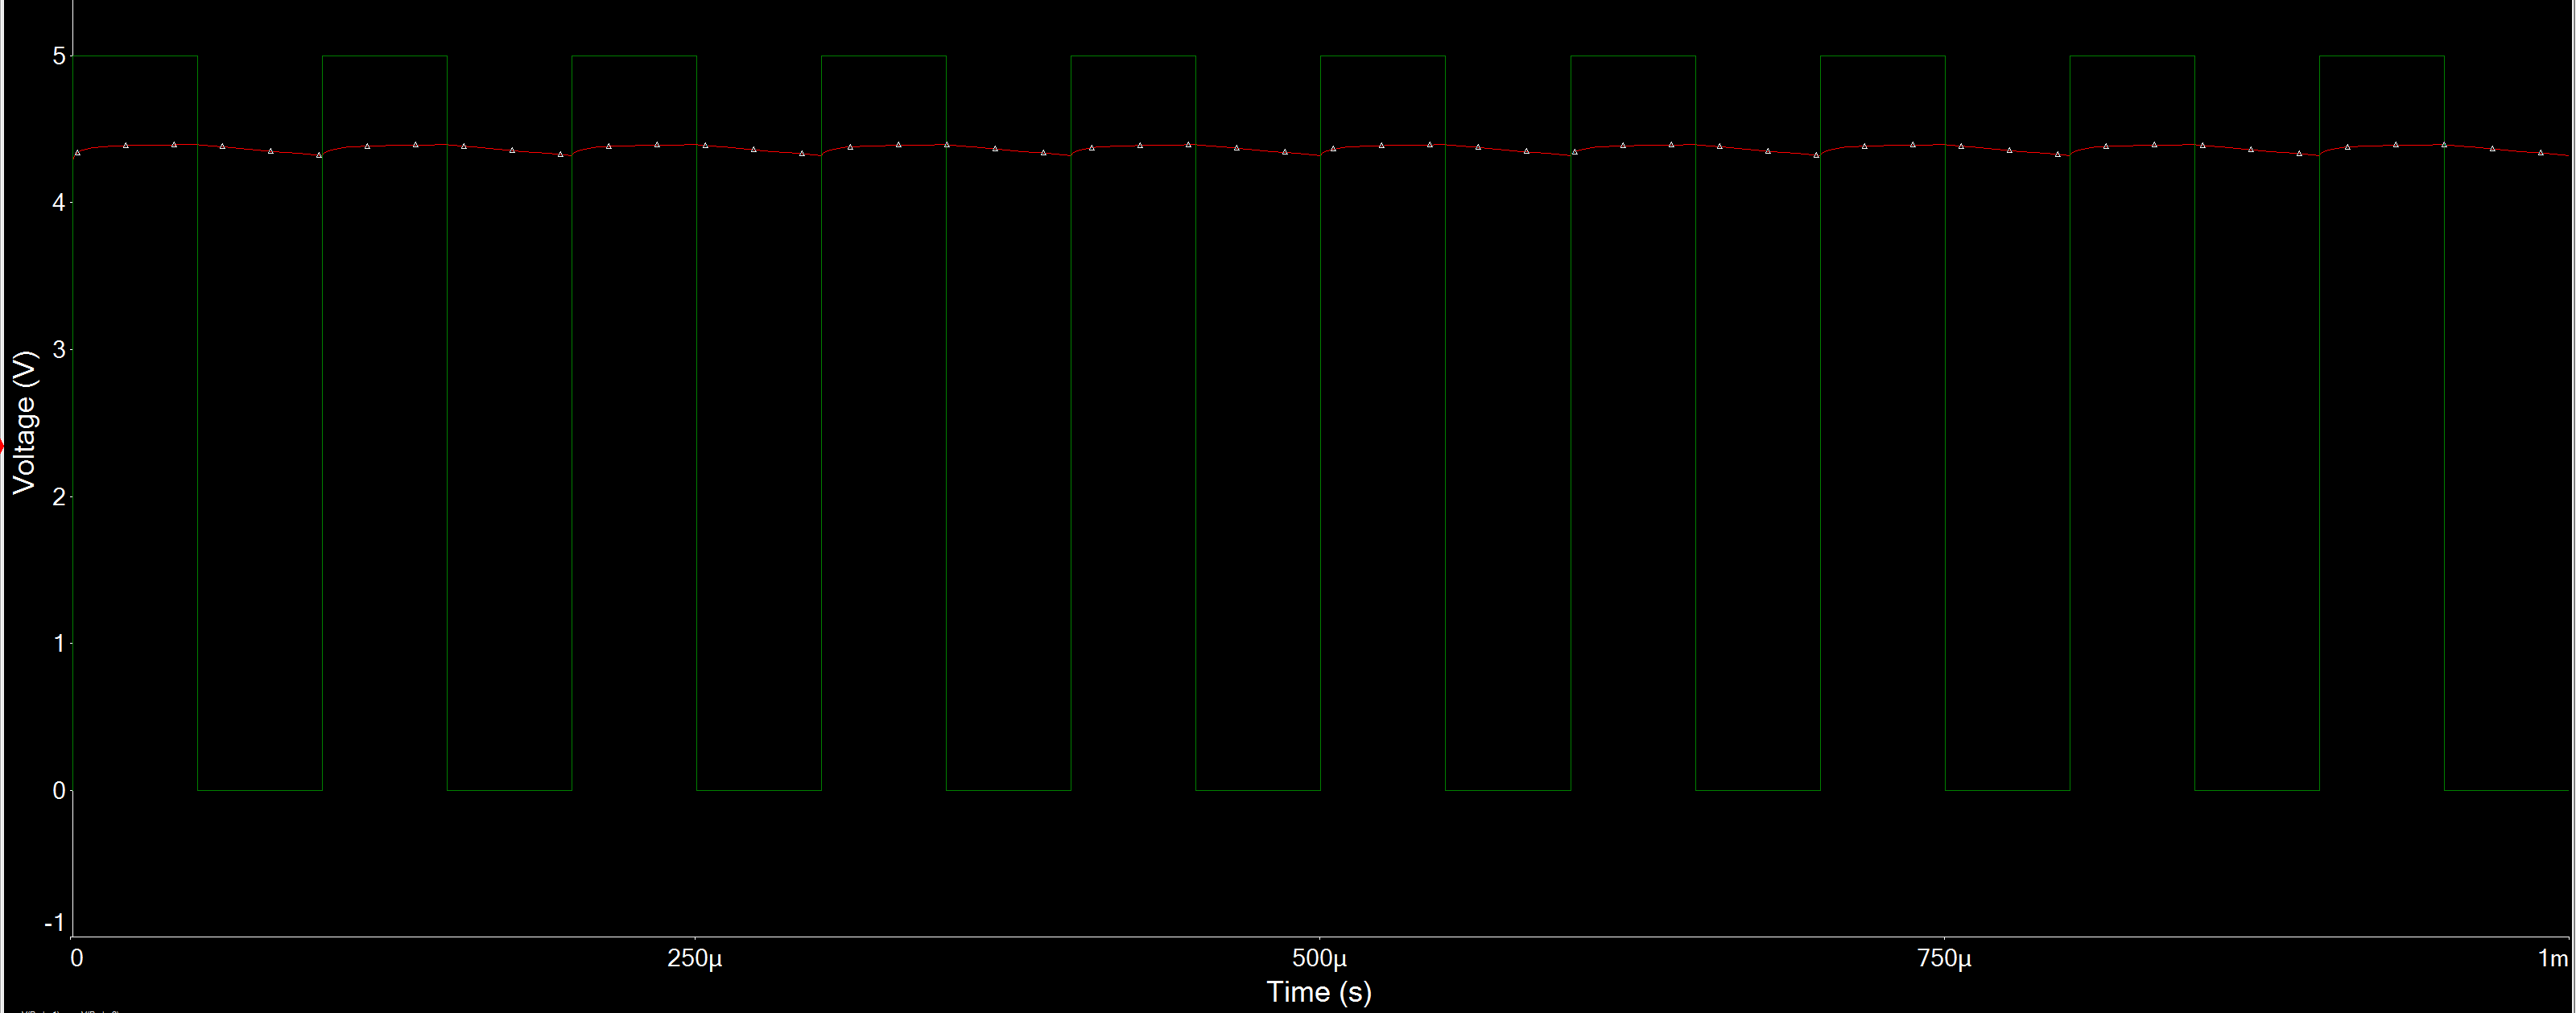
\includegraphics[width=\textwidth]{Afsnit/DesignOgImplementering/images/envelope_detector}
	\caption{Simulering af envelope detectoren}
	\label{fig:envdetsim}
\end{figure}

På simuleringen ses det, at envelopedetektoren virker, da det fremgår, at kondensatoren ikke når at aflade, inden der kommer en ny puls fra PWM-signalet. Derudover ses det også, at den når at lade op inden den første puls fra PWM-signalet kommer. Det betyder, at det signal der kommer ud ligger på cirka 4,3V. 

Outputtet fra envelopedetektoren var dog noget lavt. HEJ. Det lå mellem 1,5V og 2V. Derfor blev der indsat en ikke-inverterende forstærker for at fordoble signalet. Forstærkeren består af en opamp og to modstande. For at eftervise, at signalet fordobles, hvis de to modstande i forstærkerkredsløbet er ens, blev følgende beregning foretaget: \ref{reference til Tores bog}: 

%%%%%Spændingsdeler, forstærker%%%%%%%%%%
\begin{align}
U_{O}&=(1+\frac{R_{2}}{R_{1}}) \cdot U_{P} \\ 	\nonumber
\Rightarrow U_{O}&=(1+\frac{10k\Omega}{10k\Omega}) \cdot 2V = 4V \\	\nonumber 
\end{align}

Herefter var det muligt at aflæse et tydeligt firkantsignal med en peak-to-peak-værdi på 3,5V. 

Den røde LED er koblet direkte til et 0-5V, 10 kHz PWM-signal fra PSoC'en. Den kan godt klare sig uden en formodstand. 

Der kunne overvejes at indsætte en kondensator fysisk tæt på systemet og parallelt med R1 og fotodioden. Denne ville sikre, at VCC-niveauet opretholdes, hvis der pludselig skete et fald i VCC. 

\subsubsection{Motorstyring}
Til at styre affyringsmekanismens motor er der bygget et kredsløb med en MOSFET af typen IRLZ44 som primære komponent. Denne skal fungere som en switch, da den skal sørge for, at motoren kun kører, når der bliver sendt PWM-signal ind i den. Kredsløbsdiagrammet kan ses på figur \ref{fig:affyringsmotor}. 

\begin{figure}[H]
	\centering
	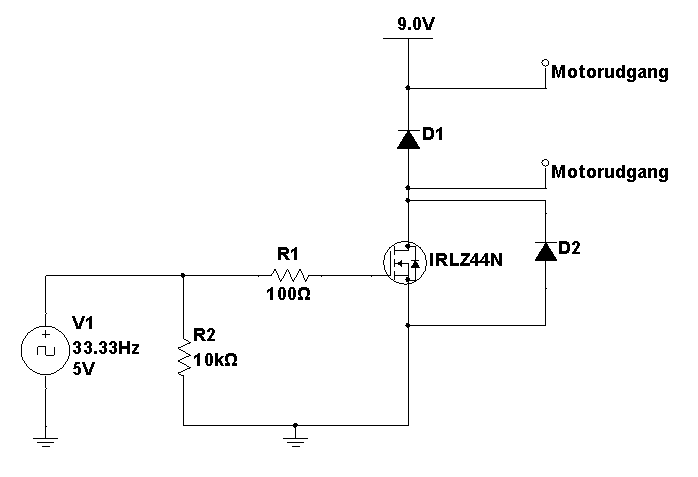
\includegraphics[width=0.7\textwidth]{Afsnit/DesignOgImplementering/images/affyringsmotor}
	\caption{Diagram over motorstyring til motor på affyringsmekanisme}
	\label{fig:affyringsmotor}
\end{figure}

Der ønskes i dette tilfælde at kunne styre motorens hastighed. Derfor anvendes et PWM-signal, som sendes ind på gatebenet og styrer motoren. Hastigheden kan så styres ved hjælp af PWM-signalets dutycycle. Hvis ikke MOSFET'en var der, ville motoren køre med fuld hastighed hele tiden, hvilket i dette tilfælde ikke ville være optimalt. 

Dioden D1 er sat ind for at sikre motoren mod store spændingsspikes, der kan forekomme, når MOSFET'en bliver afbrudt. Dioden D2, der sidder fra source til drain, sikrer, at spikes genereret af motoren, når den slukkes, ikke brænder MOSFET'en af. 

Modstanden R2 er en pull-down-modstand. Den hjælper altså til at trække de små spændinger til stel, når PWM-signalet er slukket. Når PWM-signalet er tændt, er den stor nok til, at strømmen ikke vil løbe til stel. Modstanden R1 skal sørge for, at der ikke kommer til at være en spænding på 9V på microprocessoren. Dette kunne ske, hvis der sker en kortvarig fejl i MOSFET'en. 

\subsubsection{Kanon og platform}
Selve kanonen og platformen, den står på, er bygget op af to træplader og LEGO. Den ene træplade kan dreje fra side til side, således at det er muligt at sigte i den horisontale retning. Opbygningen ses på figur \ref{fig:Horisontalmekanik}. Træpladen placeres på den øverste metalskive omkring skruen, så den drejer med rundt, når motoren roterer. Rotationen er opnået ved, at skruen kan dreje frit, men stadig er holdt lodret. Det store tandhjul er boret ud i midten, og der er indsat en møtrik, så den kan skrues på skruen. Forholdet mellem det store og det mellemste tandhjul gør, at rotationshastigheden bliver gearet ned med et forhold på 1:0,6. Forholdet er fundet ved hjælp af følgende beregning: 

\begin{align}
	gearing&=\frac{t_{m}}{t_{s}} \\ \nonumber
	gearing&=\frac{24}{40}=0,6
\end{align}

Her er $t_{m}$ antallet af tandhjul på det mellemste tandhjul og $t_{s}$ er antallet af tandhjul på det store tandhjul. 

Endeligt er motoren skruet fast til den nederste træplade, men i en højde, der gør, at den kan drive det lille tandhjul, som er forbundet med gearkæden til det store tandhjul. 

\begin{figure}[H]
	\centering
	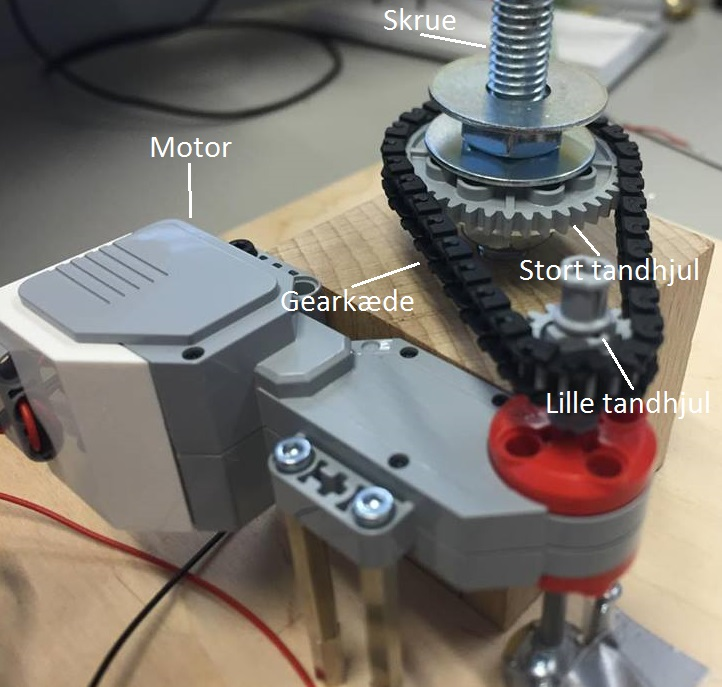
\includegraphics[width=1\textwidth]{Afsnit/DesignOgImplementering/images/horisontalMekanik}
	\caption{Horisontal mekanik}
	\label{fig:Horisontalmekanik}
\end{figure}

Mekanikken for den vertikale retning er bygget af LEGO. Et billede af opbygningen ses på figur \ref{fig:kanon}. Styringen af den vertikale bevægelse bliver håndteret af den vertikale motor, som ses på figur \ref{fig:kanon}. Motoren er forbundet til tandhjulene til vertikal styring. Der er ét tandhjul på hver side af motoren. De er begge bygget sammen med resten af kanonen. Når motoren drejer, bliver tandhjulene og hele kanonen vippet fremover eller bagover. 

Ligesom den vertikale styring er selve kanonen også bygget i LEGO. Den har et magasin, som det fremgår af figur \ref{fig:kanon}. Der kan kommes slik i magasinet, som så bliver affyret. Affyringen styres af den anden motor på figur \ref{fig:kanon}. Når affyringsmotoren drejer bliver to større tandhjul roteret. De to tandhjul er desuden forbundet til to små tandhjul, som er 5 gange så små. Med denne gearing roterer de små tandhjul 5 gange så hurtigt. De små tandhjul er forbundet til to mellem størrelse tandhjul, som drejer med dem rundt. Tandhjulene i mellemstørrelse styrer affyringen ved at omdanne den roterende bevægelse til en vandret bevægelse frem og tilbage, som affyrer kanonen.

\begin{figure}[H]
	\centering
	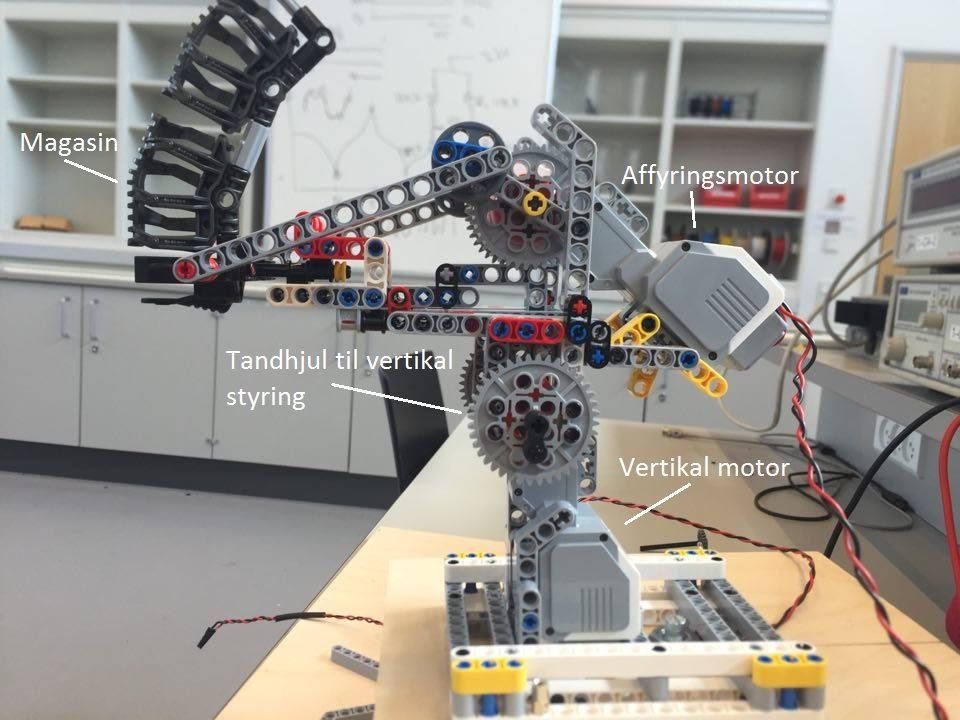
\includegraphics[width=1\textwidth]{Afsnit/DesignOgImplementering/images/kanon}
	\caption{Kanon i LEGO}
	\label{fig:kanon}
\end{figure}

For at beregne hvor stor gearing der er mellem de forskellige tandhjul opstilles nogle beregninger. Her defineres $t_{s}$ til at være antallet af tænder på det store tandhjul, $t_{m}$ er antallet af tænder på det mellemste tandhjul og $t_{l}$ er antallet af tænder på det mindste tandhjul. På figur \ref{fig:kanonOppefra} ses, hvilke tandhjul der henvises til. 

\begin{figure}[H]
	\centering
	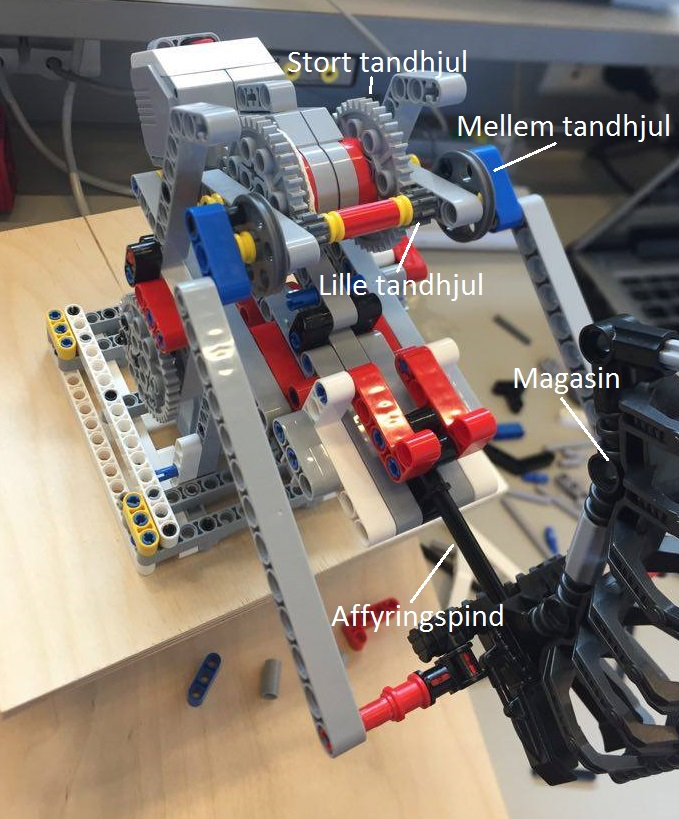
\includegraphics[width=1\textwidth]{Afsnit/DesignOgImplementering/images/kanonOppefra}
	\caption{Kanon i LEGO set oppefra}
	\label{fig:kanonOppefra}
\end{figure}


Forholdet mellem det store og det lille tandhjul er fundet ved beregningen 

\begin{align}
	gearing&= \frac{t_{s}}{t_{l}} \\ \nonumber 
	gearing &= \frac{40}{8}=5
\end{align}

Med denne gearing, får kanonen mulighed for at skyde 5 gange så kraftigt, som den ville have gjort uden gearing. 









